\documentclass[12pt, a4paper]{report}

\usepackage[utf8]{inputenc}
\usepackage[ngerman]{babel}
\usepackage{hyperref}
\usepackage{a4wide}
\usepackage{times}
\usepackage{pdfpages}
\usepackage{tabularx}
\usepackage[section]{glossaries}
\usepackage{todonotes}
\usepackage{multicol}

%graphics
\usepackage{wrapfig}
\usepackage{graphicx}
\usepackage{float}


\makeglossaries
\setcounter{tocdepth}{1} % Inhaltsverzeicnis wird nur bis \section erstellt


\date{\today}
\title{Studienarbeit Mobile Quiz}
\author{Andrea Hauser und David Windler}



\begin{document}
	
	\begin{titlepage}
		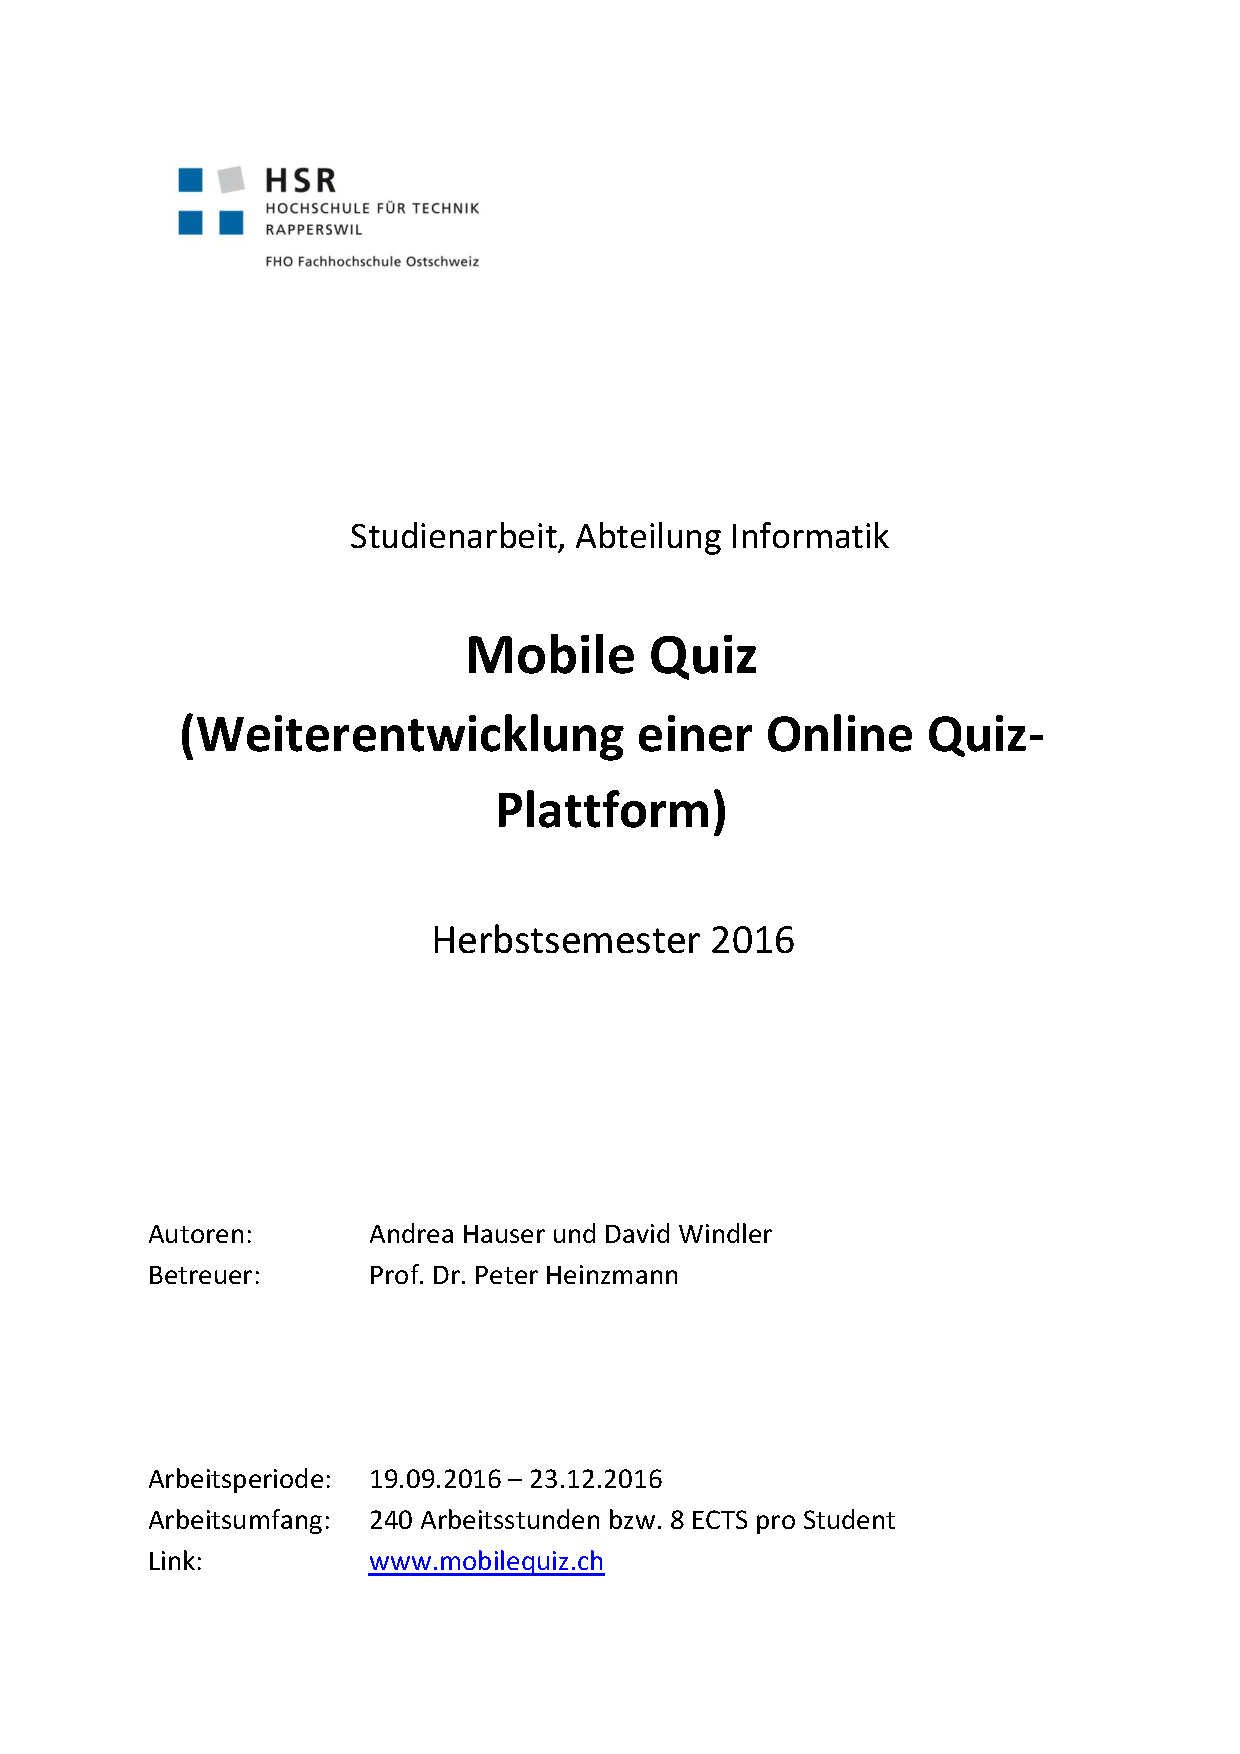
\includepdf{Titelblatt}
	\end{titlepage}
	
		
	\part{Übersicht}
	
	
	\chapter{Abstract}
	%Die Kurzzusammenfassung (Abstract) richtet sich an Leute, die den Themenkreis der Arbeit relativ gut kennen. Für diese Leute beschreiben Sie die neuen, eigenen Resultate der Arbeit. Die Kurzzusammenfassung soll nur etwa 200 Worte (etwa 20 Zeilen) lang sein. Bei Studienarbeiten ist das von der HSR Schulleitung vorgegebene Kurzzusammenfassungsformular zu verwenden.
	
	\section{Ausgangslage}
	
	
	\section{Vorgehen}
	
	
	\section{Technologien}
	
	
	
	\section{Ergebnis}
	
	
	
	
	
	\chapter{Änderungsnachweis}
	\begin{tabularx}{\linewidth}{|c|X|c|c|}
		\hline
		\textbf{Version} & \textbf{Änderungsgrund} & \textbf{Kürzel} & \textbf{Datum} \\
		\hline
		1.0 & Erstellung des Dokuments & dwi & 08.10.2016 \\
		\hline
		1.1 & Ausarbeitung 8.4 Usability & dwi & 09.10.2016 \\
		\hline
		1.2 & Titelblatt & dwi & 15.10.2016 \\
		\hline
		1.3 & Kapitel 26 Kontaktadressen, \newline Kapitel 21 Risikomanagement & ah & 15.10.2016 \\
		\hline
		1.4 & Kapitel 8 Analyse: Einleitung und Eigene Untersuchungen & dwi & 16.10.2016 \\
		\hline
		1.5 & Kapitel 8 Analyse: Recherche/ähnliche Arbeiten & ah & 16.10.2016 \\
		\hline
		1.6 & Kapitel 23 Verwendete Werkzeuge & dwi & 21.10.2016 \\
		\hline
		1.7 & Kapitel 23 Vervollständigung Verwendete Werkzeuge & dwi & 22.10.2016 \\
		\hline
		1.8 & Kapitel 21.2.2 Meilensteine beschreiben & dwi & 22.10.2016 \\
		\hline
	\end{tabularx}
	
	\listoftodos
	
	
	\tableofcontents
	%Im Inhaltsverzeichnis sollen Sie nur die Stufen Kapitel (h.), Unterkapitel (h.i) bzw. im Anhang die Haupt- (X) und Unterabschnitte (X.n) aufführen.
	
	
	\chapter{Aufgabenstellung}
	%Die unterschriebene Aufgabenstellung des Dozenten.
	
	
	
	
	\chapter{Erklärung zur Urheberschaft}
	%Unterschriebenes Formular "Erklärung zur Urheberschaft" Handelt es sich um eine Fortsetzung einer Studienarbeit, so ist in der HSR_Erklaerung_Urheberschaft klar aufzuzeigen, was im Rahmen der Studienarbeit und was bei der Bachelorarbeit gemacht wurde. In diesem Formular ist auch anzugeben, welche Informationen Copyright geschützt sind und daher nicht ohne Weiteres weitergegeben werden können.
	
	
	
	
	\chapter{Vereinbarung zur Verwendung und Weiterentwicklung der Arbeit}
	%Unterschriebenes Formular "Vereinbarung zur Verwendung und Weiterentwicklung der Arbeit".
	
	
	
	\chapter{Management Summary (Zusammenfassung)}
	%Das "Management Summary" bzw. die Zusammenfassung richtet sich in der Praxis an die "Chefs des Chefs", d.h. an die Vorgesetzten des Auftraggebers (diese sind weniger tief in die Thematik involviert als die direkt Beteiligten). Das Management Summary soll maximal 4 Seiten umfassen und mindestens eine Figur enthalten. Die Sprache soll knapp und klar sein.
	
	%Im Management Summary braucht es keine Untertitel. Die jetzt erstellten Titel sind eher als Vorgabe für den Ablauf gedacht.
	
	
	%Ausgangslage
	%	·         Ausgangslage (Warum wurde das Projekt durchgeführt? Was machen andere und welche ähnlichen Arbeiten gibt es zum Thema? Welche Ziele wurden gesteckt (Muss-, Soll-, Nice-to-Have Ziele)
	
	
	%Vorgehen
	%   ·         Vorgehen (Was wurde gemacht? In welchen Teilschritten? Wer war involviert (Durchführung, Entscheide, Zwischenprüfungen/Feedbacks usw.)? Verwendete Werkzeuge)
	
	
	%Ergebnisse
	%   ·         Ergebnisse (Was ist das Resultat des Projekts (quantifizierbarer und qualitativer Nutzen)? Was musste man selbst tun, was konnte von anderen verwendet werden? Selbstbeurteilung der  Zielerreichung in Bezug auf die Zielsetzungen der Arbeit. Abweichungen von den Zielsetzungen und Begründung dafür (positiv und negativ). Kosten. Lernpunkte aus der Durchführung des Projekts)
	
	
	%Ausblick
	%   ·         Ausblick (Verbleibende Probleme, Risiken und Gegenmassnahmen, was würde man anders machen? Wie geht es mit dem Projekt weiter, wer nutzt was? Welche weiteren Schritte, Entwicklungen, Anpassungen etc. werden empfohlen / sind geplant?)
	
	
		
	
	
	
	
	
	\part{Hauptbericht}
	
	\chapter{Einleitung}
	% !TEX root = Projektdokumentation.tex

% 	Die Einleitung soll allgemein verständlich sein, d.h. sie soll beispielsweise auch für Ihre Freunde und Verwandten verständlich sein. Sie stellt die Aufgabe in einen grösseren Zusammenhang und liefert eine genaue Beschreibung der Ausgangslage und Problemstellung. Allfällige Vorarbeiten oder ähnlich gelagerte Arbeiten sind diskutiert. Zum Schluss der Einleitung können Sie auch beschreiben, welche Abschnitte des Berichts sich an welche Leser wenden (z.B. Anwender des Produkts, Entwickler, Betreiber).

%Überprüfen von Wissen \\
Während dem Studium werden viele Inhalte vermittelt und anschliessend mit einer Schlussprüfung abgeholt. Wie merkt ein Student aber schon vor der Prüfung, ob sein Wissen sattelfest ist? Mobile Quiz bietet eine Lösung dafür. Der Dozent erfasst Fragen, mit welchen die Studenten anschliessend ihren Wissensstand ermitteln können. \\
%Stand Mobile Quiz \\
Stand heute umfasst Mobile Quiz inzwischen einige Funktionen, um Quizzes zu erstellen. Verbesserungspotentiale liegen allerdings noch in den Bereichen der Bedienbarkeit, im Bereich von neuen Fragetypen sowie in der Auswertung von Quizzes. Durch letzteres wäre es dem Dozenten ersichtlich, welche Teile des Stoffs gut verstanden wurden und bei welchen noch Nachholbedarf herrscht. Somit könnte die Vorlesungszeit effizienter genutzt werden.
\\
%In dieser Arbeit wird XY umgesetzt.
\\
%Übersicht Kapitel \\
	
	\todo{Andrea}
	
	
	%Die nach der Einleitung folgenden Hauptabschnitte richten sich in der Regel an die Nutzer und Betreiber des realisierten Systems und an die im entsprechenden Fachgebiet tätigen Ingenieure. Die Hauptabschnitte bilden typischerweise die wichtigsten Ergebnisse Ihrer Arbeit ab. Sie beschreiben das realisierte System bzw. die getätigten Untersuchungen. Die Leser sollen die zur Problemlösung getätigten Überlegungen verstehen. Theoretische Grundlagen sind soweit aufzuführen, als dies für die Lösung der Aufgabe nötig ist (keine Lehrbücher oder Wikipedia-Artikel (ab)schreiben). Die Erkenntnisse aus den theoretischen Untersuchungen sind also wenn immer möglich direkt mit der Problemlösung zu verknüpfen (z.B. mit eigenen Messungen oder mit Beispielen aus der schliesslich erstellten Anwendung zu illustrieren).
	
	%Sparen Sie nicht mit Diagrammen und Figuren. Diese müssen auch im Text diskutiert sein, d.h. es wird auch in Worten beschrieben, was man mit dem Diagramm oder der Figur zeigen will. Spezielle Details, welche die Kontinuität in den Hauptabschnitten stören, sind im Anhang aufzuführen.
	
	%Der Umfang der einzelnen Abschnitte des Berichts entspricht in der Regel dem Arbeitsaufwand, welcher für die entsprechenden Themen eingesetzt wurde.
	
	%Je nach Aufgabenstellung können beispielsweise Hauptabschnitte der folgenden Art vorkommen:
	
	\chapter{Analyse}
	% !TEX root = Projektdokumentation.tex


\newglossaryentry{Cross-Site-Scripting}{name={Cross-Site-Scripting},description={
		Cross-site scripting (XSS) ist ein Angriff auf eine Webapplikation, die Benutzereingaben nicht sorgfältig überprüft, bevor diese wieder an weitere Benutzer zurückgeschickt werden. So kann ein Angreifer ausführbaren Code mitgeben, der anschliessend bei vielen anderen Benutzern im Browser ausgeführt wird \cite{whatIs_xss}}}

\newglossaryentry{Vulnerability}{name={Vulnerability},description={
		Fehler im Code oder Design, welcher ein potentielles Sicherheitsrisiko darstellt \cite{whatIs_vulnerability}}}

\newglossaryentry{CSV}{name={CSV},description={CSV steht für Comma-Seperated Values und ist ein Textformat.}}

\newacronym{IKF}{IKF}{Institut für Kommunikation \& Führung}

\newacronym{SKMF}{SKMF}{Swiss Knowledge Management Forum}

%Analyse der Aufgabenstellung, Requirements Engineering, Umfeldanalyse (vergleichbare Produkte und Lösungen), Resultate der Literaturrecherche
%Auch: Ziel und Zweck von Mobile Quiz, wofür und vom wem wird es eingesetzt? Was ist zukünftiges Ziel?

% Hier werden alle Erkenntnisse aus den einzelnen Unterkapitel zusammengefasst.
%ohne Titel

Um ein möglichst gutes Bild davon zu erhalten, was im Bereich Online-Quizzes bereits vorhanden ist und wo Mobile Quiz aktuell steht, wurden Informationen in verschiedenen Bereichen gesucht und zusammengetragen.

\bigskip

Dazu wurden unter anderem ähnliche Arbeiten, im Sinne von Bachelorarbeiten oder Studienarbeiten, gesucht (Abschnitt \ref{sec:rechercheAehnlicheArbeiten}) und diese auf ihre Relevanz überprüft. Dabei wurde festgestellt, dass sich, was Arbeiten von Studierenden betrifft, vor allem die HSR auf Quizzes im Lernbereich konzentriert. Andere Hochschulen befassten sich vor allem mit Online-Plattformen, welche auf Prüfungssituationen ausgelegt sind. Da es sich dabei um unterschiedliche Anwendungsbereiche mit unterschiedlichen Anforderungen handelt, wurden diese Arbeiten nicht im Detail angeschaut.

\bigskip

Das Testen von Mobile Quiz selbst (Abschnitt \ref{subsec:eigeneUntersuchungen}) zeigte, dass es noch einige Probleme in der Version 3 anzutreffen gab. Diese zu beheben würde die Plattform solider machen und bestenfalls neue Quiz-Ersteller anziehen.
Weiter wurde beim Vergleich mit anderen Online-Quiz-Plattformen (Abschnitt \ref{subsec:Webuntersuchungen}) ersichtlich, dass Mobile Quiz im Bereich Funktionsumfang und Einstellungsmöglichkeiten gut dastand. Allerdings konnte Mobile Quiz im Bereich Usability nicht Punkten, da viele Funktionen nicht sofort ersichtlich oder nur schwierig zu erreichen waren. Dies wurde auch durch die Usability-Tests (Abschnitt \ref{sec:usability}) bestätigt, welche ebenfalls zu Beginn der Arbeit durchgeführt wurden.

\bigskip

Die Ergebnisse aus dieser Untersuchung flossen zusammen mit den bereits bekannten Verbesserungspunkten in die Aufgabenstellung dieser Studienarbeit ein und sind im Anhang unter \glqq MoeglicheArbeitenSA\grqq ab Seite \pageref{pdf:moeglicheArbeiten} ersichtlich. Um nicht jeden Fehler einzeln aufzuführen, wurden darin die Probleme abstrahiert und nur Themenbereiche aufgeführt und beschrieben. Diese wurden zusammen mit dem Betreuer nach ihrer Wichtigkeit priorisiert.

\newpage

\section{Recherche/ähnliche Arbeiten}
\label{sec:rechercheAehnlicheArbeiten}

Welche ähnlichen Arbeiten, seien es Bachelorarbeiten, Studienarbeiten oder sonstige Arbeiten mit ähnlichem Themenbezug, gibt es bereits?

Um möglichst viele Quellen zu berücksichtigen wurde bei der Bibliothek das Angebot \glqq Book a Librarian\grqq \cite{hsr_book_a_librarian} in Anspruch genommen. Die mitgenommenen Tipps wurden für weitere Arbeiten im Dokument \glqq Recherchetipps\_book-a-librarian\grqq ab Seite  festgehalten. Dieses Dokument ist im Anhang unter \glqq Recherchetipps von Book a Librarian\grqq zu finden. Die allgemeinen Recherchetipps der Bibliothek sind unter folgender URL erreichbar: \url{https://www.hsr.ch/fileadmin/user_upload/customers/hsr/HSR-INTERN/Bibliothek/Bibliothek_Startseite/Recherchetipps_Dossier.pdf}

\bigskip

Da es kein zentrales, Schulen-übergreifendes Verzeichnis aller Arbeiten gibt, musste zur Beantwortung dieser Frage die einzelnen Verzeichnisse der Schulen durchgegangen werden. Dabei wurden die folgende Schulen, aufgelistet mit dem jeweiligen gefundenen Ergebnissen, beachtet:
\begin{itemize}
	\item ETH Zürich
	\begin{itemize}
		\item Die Arbeiten, welche an der ETH Zürich erstellt wurden, behandeln spezifisch auf die Prüfungssituation ausgelegte Tools. Diese Arbeiten wurden deshalb nicht weiter im Detail betrachtet. \cite{zeller_automated_2014} \cite{antonucci_autoteach_2014} \cite{heinrich_design_2008} \cite{nanzer_einsatz_2005}
	\end{itemize}
	\item ZHAW
	\begin{itemize}
		\item Im Verzeichnis aller Arbeiten stach die Arbeit \glqq Edu4u. Geschäftsmodell einer Webplattform im E-Learning-Bereich für E-Lectures, Online-Kurse und Filmdokumentationen\grqq heraus. Leider konnte diese Arbeit nicht genauer angeschaut werden, da sie als vertraulich klassifiziert wurde. \cite{_bachelorarbeiten-2013-zhaw-sml.pdf_}
	\end{itemize}
	\item Universität Zürich
	\begin{itemize}
		\item Hier wurde leider kein Verzeichnis der Arbeiten gefunden.
	\end{itemize}
	\item HSR
	\begin{itemize}
		\item Bachelorarbeit \glqq Digital Native Quiz\grqq \cite{grob_digital_2010} aus dem Jahr 2010, mit Prof. Dr. Peter Heinzmann als Betreuer.
		\item Bachelorarbeit \glqq MobileQuiz\grqq \cite{khalid_bachelorarbeit_mobile_quiz_juni_2012.pdf_2012} aus dem Jahr 2012 mit Prof. Dr. Peter Heinzmann als Betreuer. Dabei handelt es sich um die Vorgängerarbeit zu dieser Studienarbeit.
		\item Studienarbeiten \glqq Crowdsourced Quizzes\grqq \cite{_technischer_bericht-quizzenger_crowdsourced_quizzes.pdf_} und \glqq Crowdsourced Quizzes 2\grqq \cite{_technischer_bericht-quizzenger-2.pdf_} aus den Jahren 2014 und 2015, jeweils mit Prof. Frank Kock als Betreuer. Als Ergebnis entstand der Quizzenger, ein Online-Quiz-Tool, welches viel Wert auf Gamification, also das spielerische Lernen legt.
	\end{itemize}
\end{itemize}


Von den gefundenen Arbeiten konnte keine für die Lösung von spezifischen Fragestellungen als Nachschlagewerk verwendet werden. Die Arbeiten, welche von Prof. Dr. Peter Heinzmann betreut wurden, waren schon in Mobile Quiz integriert, andere Arbeiten wiesen einen anderen Einsatzzweck auf.

Bei der Suche nach ähnlichen Arbeiten, wurde auch der Standard \glqq IMS Question \& Test Interoperability\grqq \cite{imsglobal.org} der IMS Global Learning Consortium entdeckt. Dieser Standard beinhaltet eine umfassende Übersicht von möglichen Fragetypen.

Das IMS Global Learning Consortium setzt sich allgemein dafür ein, dass ein gemeinsamer Standard zur Repräsentation von Fragen entsteht, um für Interoperabilität zwischen einzelnen Lernseiten zu sorgen. Bei vertieften Abklärungen wurde festgestellt, dass sowohl Moodle \cite{moodle} als auch TAO \cite{tao} (zwei der Open Source Seiten, welche in der Webuntersuchung angeschaut wurden) sich auf die Standards von IMS Global Learning Consortium ausrichten.

Es wurde entschieden nicht auf die Standards von IMS Global zu wechseln, da es sich um einen zu grossen Aufwand handeln würde. Zudem ist für MobileQuiz auf absehbare Zeit kein Austausch mit anderen Lern-Webseiten vorgesehen.


\section{Eigene Untersuchungen, Webuntersuchung}
\label{sec:eigeneUntersuchungenWebuntersuchungen}

Was kann Mobile Quiz heute bereits, wo gibt es noch Probleme und wo steht das Quiz heute im Vergleich zu ähnlichen Webanwendungen? Diese Fragen waren Kern der eigenen Untersuchungen. Einerseits wurde dazu Mobile Quiz selbst intensiv getestet, andererseits wurden mehrere vergleichbare Online-Quizzes gesucht und diese anhand von vorher definierten Kriterien verglichen.


	\subsection{Untersuchung www.mobilequiz.ch}
	\label{subsec:eigeneUntersuchungen}
	Während mehrerer Stunden wurden sowohl in der Rolle als Lernender, welcher ein Quiz nutzt, in der Rolle als Ersteller, welcher ein neues Quiz erstellt, und in der Rolle des Administrators, welcher Zugriff auf alle Inhalte hat und auch andere Benutzer verwalten kann, die vorhandenen Funktionen ausprobiert. Dabei kamen verschiedene Probleme zutage, die sich grob in die folgenden Kategorien unterteilen lassen:
	
	
	\begin{itemize}
		\item Sicherheitsrelevante Probleme \\
		Dabei handelt es sich um sämtliche Probleme, welche ein Angreifer ausnutzen kann, um unberechtigte Aktionen durchzuführen. \\
		\textit{Beispiel}: Wird eine Frage erfasst, so kann im Fragetext mittels HTML-Script-Tag JavaScript hinterlegt werden, welches beim Anzeigen der Frage beim Teilnehmer ausgeführt wird. Somit hat Mobile Quiz gegenüber Frage-Erstellern eine \gls{Cross-Site-Scripting} - \gls{Vulnerability}. Diese kann ausgenutzt werden, um das Session-Cookie eines Benutzers zu stehlen. Dabei handelt es sich um ein grosses Risiko, denn sobald ein Angreifer das Session-Cookie eines Benutzers hat, kann er sich als diesen ausgeben. Das Worst-Case Szenario für das Mobile Quiz ist, dass sich jemand an der Prüfung als ein anderer Benutzer ausgibt, oder einem anderen Benutzer die Quiz-Teilnahme sabotiert.
		
		
		\begin{figure}[H]
			\centering
			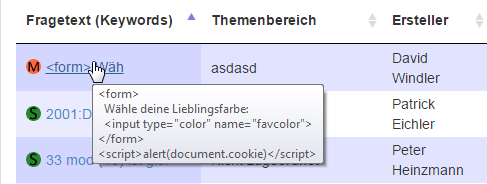
\includegraphics[width=0.7\textwidth
			]{Images/XSS_Frage.PNG}
			\caption{Platzierung des Script-Tags in der Frage}
			\cite{mobilequiz.ch}
		\end{figure}
		
		\begin{figure}[H]
			\centering
			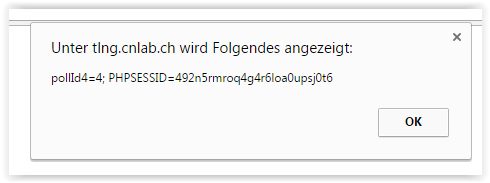
\includegraphics[width=0.7\textwidth
			]{Images/XSS_Cookie.PNG}
			\caption{Anzeige des Cookie beim Lösen der Frage}
			\cite{mobilequiz.ch}
		\end{figure}
		
		
		\item Usability \\
		In dieser Kategorie wurden die Probleme mit der Navigation und dem Auffinden von Funktionen zusammengefasst. \\
		\textit{Beispiel}: In der Lernkontrollen-Übersicht ist der Start-Button zu wenig ersichtlich.
		\begin{figure}[H]
			\centering
			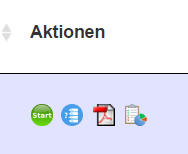
\includegraphics[width=0.20\textwidth]
			{Images/MobileQuizAlteVersionStartbutton.png}
			\caption{Ansicht der möglichen Aktionen inkl. Start-Button}
			\cite{mobilequiz.ch}
		\end{figure}
		\item Mobile-Probleme \\
		Die Kategorie beinhaltet sämtliche Probleme, welche nur in der mobilen Ansicht der Webseite vorhanden sind. \\
		\textit{Beispiel}: Der Zugriff via Smartphone auf den Profilbereich funktioniert nicht.
		\item Administrator \\
		In dieser Kategorie wurden Probleme notiert, welche nur mit Administrator-Rechten vorhanden sind. \\
		\textit{Beispiel}: Wird ein neues Themengebiet beantragt, so wird dies nicht im Log festgehalten.
		\item Probleme/Bugs \\
		In dieser Kategorie wurden alle Fehler und Probleme festgehalten, welche keiner spezifischeren Kategorie zugeordnet werden konnten. \\
		\textit{Beispiel}: Wird bei einer Lernkontrolle festgelegt, dass sie keinen Endzeitpunkt hat, so soll bei der Quiz-Teilnahme auch kein Enddatum angezeigt werden.
		\item Allgemeine Fragen zum Konzept \\
		Die Kategorie umfasst Punkte, welche zwar korrekt funktionieren, aber deren Zweck unter Umständen nicht benötigt wird. \\
		\textit{Beispiel}: Muss bei einer Registrierung wirklich die Adresse angegeben werden?
		\item Schreibfehler/Grammatik \\
		In dieser Kategorie wurden Schreibfehler oder inkonsistente Handhabungen von Ausdrücken festgehalten. \\
		\textit{Beispiel}: Der Benutzer wird wird teilweise mit \glq Sie\grq angesprochen, andernorts wird die \glq Du\grq-Form verwendet.
	\end{itemize}

	Die ausführlichen Resultate sind im Anhang unter \glqq Ergebnisse eigene Tests\grqq ersichtlich.	


	\subsection{Vergleich Online-Quizzes}
	\label{subsec:Webuntersuchungen}
	Um andere Online-Quizzes mit Mobile Quiz zu vergleichen mussten zuerst die Kriterien festgelegt werden. Als Grundlage diente eine Excel-Tabelle von Khalid Abdul und Patrik Naef, welche an die Bedürfnisse dieser Arbeit angepasst wurde. Es wurden folgende Vergleichskriterien festgelegt:
	\begin{itemize}
		\item Fragemöglichkeiten \\
		Welche Möglichkeiten bestehen eine Frage zu stellen? \\
		\textit{Beispiel:} Text mit Bild
		\item Antwortmöglichkeiten \\
		Auf welche Weise kann geantwortet werden? \\
		\textit{Beispiel:} Multiple-Choice
		\item Zeitsteuerung \\
		Gibt es Zeitbeschränkungen? \\
		\textit{Beispiel:} Festlegung der Zeit pro Frage
		\item Visuelle Signale \\
		Gibt das System Rückmeldungen an den Benutzer? \\
		\textit{Beispiel:} Rückmeldung bei Ablauf der Zeit
		\item Fragenauflösung \\
		Welche Möglichkeiten zur Punktevergabe sind vorhanden? \\
		\textit{Beispiel:} Individuelle Punktevergabe pro Frage
		\item Testfunktion \\
		Kann das Quiz vor Veröffentlichung durchgespielt werden? \\
		\item Textdarstellung \\
		Welche Einstellung können am angezeigten Text vorgenommen werden? \\
		\textit{Beispiel:} Anpassung der  Schriftgrösse
		\item Auswertungsmöglichkeiten \\
		Welche Möglichkeiten gibt es für den Ersteller das Quiz auszuwerten? \\
		\textit{Beispiel:} Auswertung pro Teilnehmer
		\item Internationalisierung \\
		Welche Möglichkeiten gibt es zur Unterstützung von mehreren Sprachen? \\
		\textit{Beispiel:} Mehrsprachige Erfassung der Quiz-Fragen
		\item Erfassen von unterschiedlichen Elementen \\
		Kann der Ersteller Kategorien, Studenten oder Gruppen erfassen?
		\item Allgemein \\
		Verschiedenen Möglichkeiten, um den Umgang mit dem Quiz zu erleichtern. \\
		\textit{Beispiel:} Erstellung eines QR-Codes zur direkten Teilnahme am Quiz
		\item Spezielle Funktionen \\
		Gibt es die Möglichkeit von Online-Kursen?
		\item Benutzerfreundlichkeit \\
		Gibt es Elemente, die dem Benutzer helfen sich leichter zurechtzufinden? \\
		\textit{Beispiel:} Schritt-für-Schritt - Erstellung eines Quizzes
	\end{itemize}
	
	\bigskip
	
	Die zu vergleichenden Websites wurden durch Google-Suchen und Empfehlungen von educatorstechnology.com \cite{educatorstechnology.com} ausgewählt.
		
	Um sicher zu sein, dass die gewählten Webseiten einen repräsentativen Anteil der Lernquizzes abdecken, wurde Kontakt mit Personen aufgenommen, welche in diesem Umfeld tätig sind. Um Unterstützung angefragt wurde bei Switch AAA, dem \acrfull{IKF} und beim \acrfull{SKMF}.
	Leider hatte bei Switch AAA niemand Zeit zur Beantwortung dieser Frage. Das \acrshort{IKF} hat selbst keine Vergleiche über bestehende Online-Quizzes, oder falls doch, handelt es sich um Unterrichtsmaterial, welches nicht herausgegeben wird. Das \acrshort{SKMF} konnte nur via ein Webformular kontaktiert werden und hat sich bis zum Ende dieser Arbeit nicht zurückgemeldet.
	
	\bigskip
	
	Die detaillierte Auswertung des Vergleichs ist im Dokument 'SA-Mobile-Quiz\_QuizSysteme-Funktionen-Vergleich-Matrix.xlsx' ersichtlich. Im Folgenden werden die wichtigsten Punkte aus dieser Analyse aufgezeigt. Es wird jeweils die Lösung im aktuellen Mobile Quiz der HSR mit der besten Lösung aus den verschiedenen Vergleichsquizzes präsentiert:
	
	\begin{itemize}
		\item Willkommensseite \\
		Webanwender haben eine riesige Auswahl an Seiten, welche auf ihr Bedürfnis zugeschnitten sind. Sie wenden deshalb nicht viel Zeit auf, um sich über eine einzelne Seite genauer zu informieren. Aus diesem Grund ist der erste Eindruck entscheidend, also eine ansprechende Willkommensseite. \\
		
		\begin{figure}[H]
			\centering
			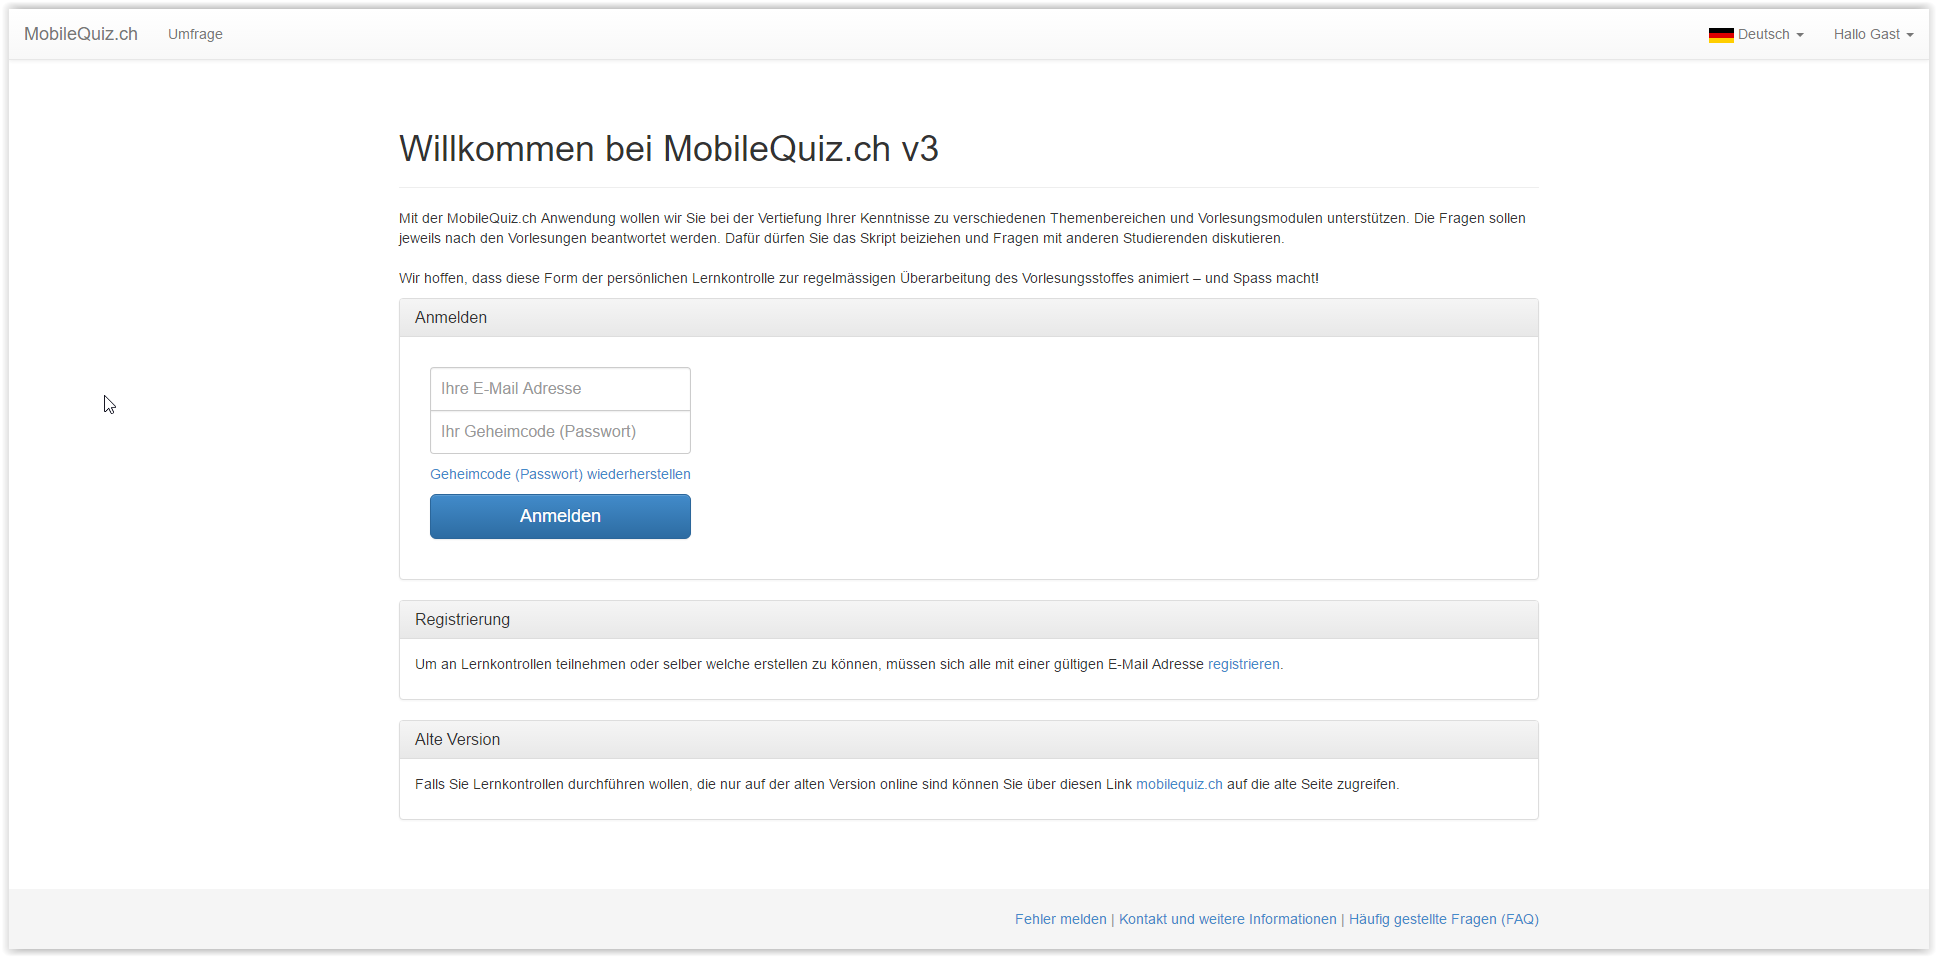
\includegraphics[width=0.75\textwidth]{Images/MobileQuiz_StartPage.PNG}
			\caption{Startseite Mobile Quiz Version 3}
			\cite{mobilequiz.ch}
		\end{figure}
		
		Ruft man www.mobilequiz.ch auf, so sieht man viel Text, der die Seite beschreibt. Ein Benutzer weiss jedoch noch nicht genau, was ihn erwartet, wenn er sich registriert und einloggt.
		
		\begin{figure}[H]
			\centering
			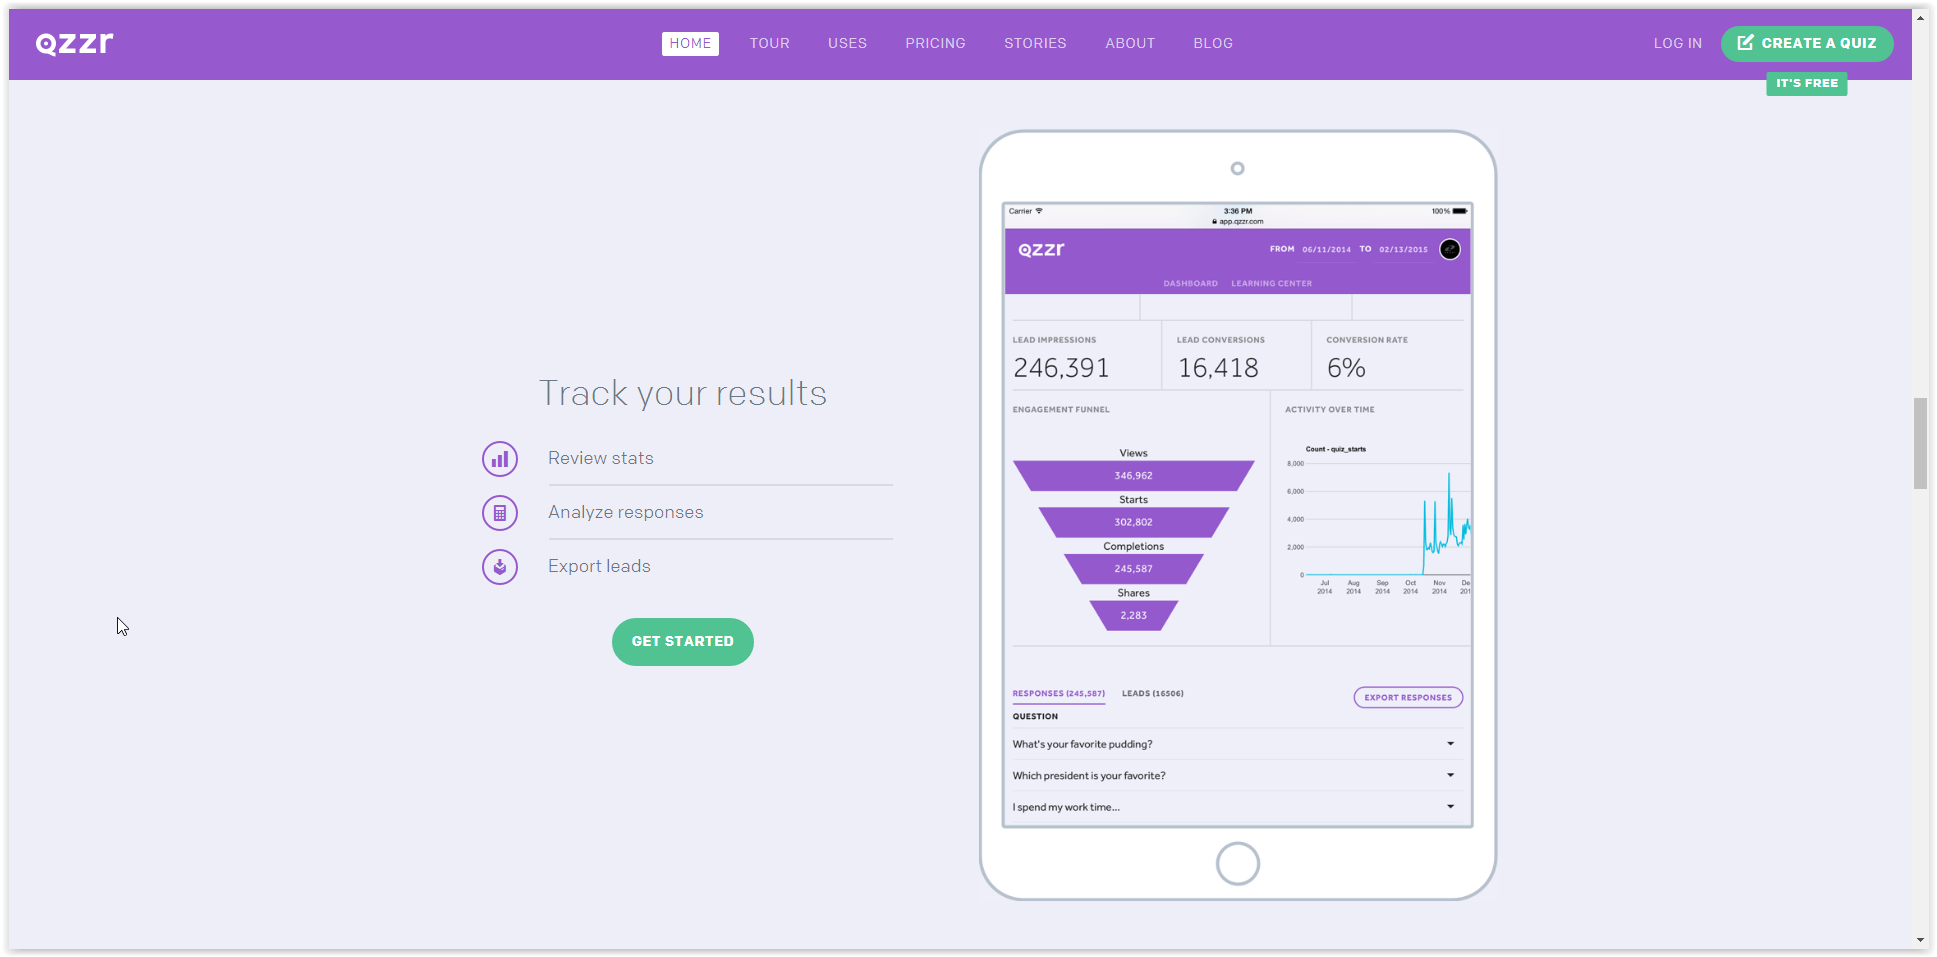
\includegraphics[width=0.75\textwidth]
			{Images/Qzzr_StartPage_Statistics.PNG}
			\caption{Startseite Qzzr}
			\cite{qzzr.com}
		\end{figure}
				
		Seiten wie Qzzr \cite{qzzr.com} hingegen, zeigen anhand von Bildern und Symbolen auf, was die Funktionalitäten sind und wie diese konkret aussehen. Solche Bilder sind schnell erfasst  und verarbeitet.
		Mobile Quiz könnte die gleichen Funktionsumfang bieten, aber wenn es der Benutzer nicht sofort sieht, klickt er weiter und registriert sich andernorts.
		
		Was machen gute Willkommensseiten also aus? \\
		Antworten darauf bietet unter anderem der Blog-Eintrag \glqq 16 of the Best Website Homepage Design Examples\grqq \cite{hubspot_kolowich} von Lindsay Kolowich.
		Aufgrund von mangelnder Zeit konnte die Willkommensseite nicht neu gestaltet werden. Dieser Punkt fliesst deshalb ins Kapitel \ref{sec:InhalteFuerStudentenarbeiten}, Inhalte für weitere Studentenarbeiten ein.
		
		
		\item Schritt für Schritt - Erstellung von Quizzes \\
		Um ein Quiz zu erstellen benötigt es einerseits die Fragen, andererseits das Quiz selbst, welches mehrere Fragen umfasst. In welcher Reihenfolge sollen diese beiden Ressourcen erstellt werden? \\
		Bei Mobile Quiz war der Ablauf so geregelt, dass zuerst die Fragen und anschliessend das Quiz separat erstellt wurde. War man sich dieser Tatsache bewusst, so stellte dies kein Problem dar, aber war es auch intuitiv? Wie in den durchgeführten Usability-Tests festgestellt wurde, war dem nicht so. Die Benutzer starteten sofort mit der Erstellung des Quizzes, mussten dann aber abbrechen, weil darin keine neuen Fragen erfasst werden konnten.
		Aus diesem Grund war es sinnvoll, diese Reihenfolge in Mobile Quiz zu ändern. Hier bot Testmoz \cite{testmoz.com} ein gutes Vorgehen:
		
		\begin{enumerate}
			\item Testnamen eingeben
			\item Testeinstellungen vornehmen
			\item Fragen erfassen
			\item Veröffentlichen
			\item Reports anschauen
		\end{enumerate}
		
		\begin{figure}[H]
			\centering
			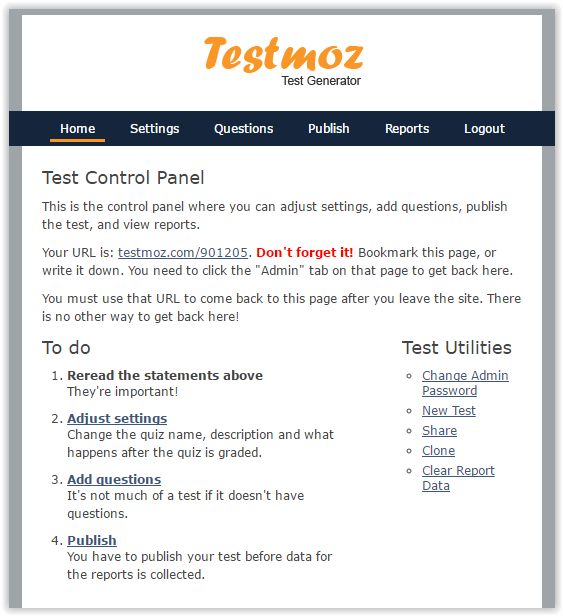
\includegraphics[width=0.4\textwidth]{Images/Testmoz2.PNG}
			\caption{Ablauf Testmoz}
			\cite{testmoz.com}
		\end{figure}
		
		Der Ablauf von Mobile Quiz war einzig darin zu ändern, dass neue Fragen während der Erstellung eines Quizzes erfasst werden können. Zur Vereinfachung konnte auch beitragen, dass der Ablauf wie bei Testmoz \cite{testmoz.com} verteilter dargestellt wird, sodass pro Seite weniger Informationen stehen. Somit findet sich der Benutzer schneller zurecht. Die genaue Beschreibung dieser Umstellung ist in Kapitel \ref{subsec:quiz-erstellung} genauer beschrieben.
		
		
		
		
		\item  Quiz-Einstellungen \\
		Quizzes können für unterschiedliche Bedürfnisse eingesetzt werden. Die möglichen Einsatzzwecke reichen von Freunden, die zum Zeitvertreib ihr Wissen gegenseitig messen wollen, über Dozenten, die prüfen möchten, ob die Studenten den Unterrichtsstoff verstanden haben, bis zu Dozenten, welche die Quizzes als Prüfung verwenden.
		Diese Situationen verlangen viele Einstellungsmöglichkeiten, welche für den Benutzer möglichst selbsterklärend sein sollen. Trifft dies jedoch nicht zu, oder ist die Darstellung unverständlich, so wird sich der Quiz-Ersteller möglicherweise nach einer anderen Quiz-Plattform umsehen.
		
		\begin{figure}[H]
			\centering
			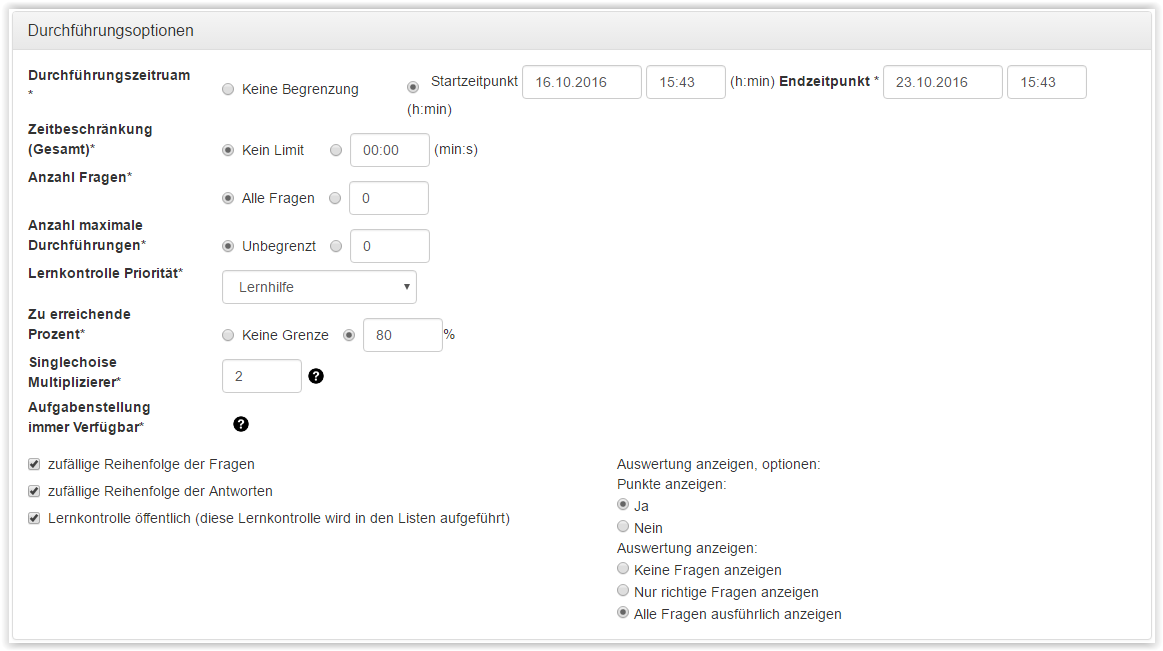
\includegraphics[width=0.75\textwidth
			]{Images/MobileQuiz_Quiz-Settings.PNG}
			\caption{Quiz-Einstellungen Mobile Quiz Version 3}
			\cite{mobilequiz.ch}
		\end{figure}
		
		
		Mobile Quiz bot zwar viele Einstellungsmöglichkeiten an, diese waren jedoch so zahlreich, dass sie den Benutzer fast überforderten. Zudem war die Darstellung zum Teil nicht optimal, da beispielsweise die 'Auswertung Anzeigen - Optionen' weiter rechts angezeigt wurde als alle anderen Einstellungen.
		
		\begin{figure}[H]
			\centering
			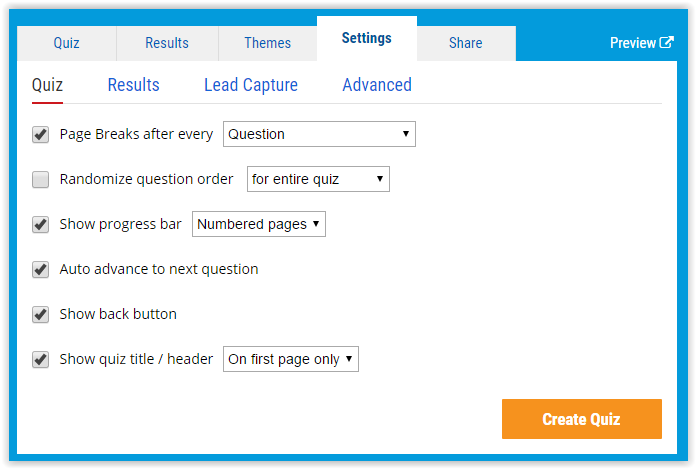
\includegraphics[width=0.5\textwidth
			]{Images/QuizMaker_Quiz-Settings.PNG}
			\caption{Quiz-Einstellungen Quiz Maker}
			\cite{quiz-maker}
		\end{figure}
		
		Aufgeräumter wirkten die Einstellungen beispielsweise bei Quiz Maker \cite{quiz-maker}. Zwar gab es ebenfalls eine Vielzahl von Möglichkeiten, diese wurden aber übersichtlich dargestellt, indem sie Themen zugeordnet und auf Tabs verteilt wurden. Zudem gab es einen eigenen Tab für erweiterte Optionen. \\
		Bei Mobile Quiz wurde der Ablauf der Quiz-Erstellung neu organisiert und in diesem Schritt auch die Quiz-Einstellungen verteilter und übersichtlicher angeordnet. Die genaue Beschreibung ist in Kapitel \ref{subsec:quiz-erstellung} vorzufinden.
		
		
		
		\item Quiz kann vor Veröffentlichung durchgespielt werden \\
		Wie sieht das erstellte Quiz für den Teilnehmer aus? Gibt es noch Rechtschreibfehler oder werden Inhalte nicht optimal dargestellt? Ein Quiz-Ersteller wird sich all diese Fragen womöglich stellen und die einfache Lösung dazu ist, dass man das Quiz vor Veröffentlichung selbst durchspielt. Die eigene Teilnahme soll jedoch nicht zählen, da sie die Auswertungsstatistik verfälschen kann. \\
		Mobile Quiz bot die Möglichkeit an, ein Quiz noch nicht zu veröffentlichen und es auf diese Weise auszuprobieren. Dies funktionierte aber nur, wenn man als Administrator eingeloggt war. Zudem zählte die eigene Teilnahme in die Gesamtauswertung mit hinein.
		Dieser Punkt konnte mangels Zeit nicht umgesetzt werden, wird aber in Kapitel \ref{sec:InhalteFuerStudentenarbeiten}, Inhalte für weitere Studentenarbeiten einfliessen.
		
		
		\item Template für Frage-Import \\
		Ist man im Zug unterwegs und möchte trotzdem an einem neuen Quiz-Fragen arbeiten, so fehlt meist der Internetzugang. Dies kompensierte Mobile Quiz dadurch, dass Fragen aus \gls{CSV}-Dateien eingelesen und erstellt werden konnten. Um dies zu nutzen, benötigte es jedoch eine spezielle Formatierung, was neue Benutzer abschrecken konnte. \\
		Die Lösung dazu war es, ein Excel-Template, also eine Vorlage, für neue Fragen bereitzustellen. Darin kann der Benutzer schnell und einfach Fragen erfassen und muss sich nicht um das Format kümmern. Solche Templates bot beispielsweise
		Socrative \cite{socrative.com} an. Es ist im Anhang unter 'socrativeQuizTemplate.xlsx' zu finden.
		
		Im Rahmen dieser Arbeit wurde ebenfalls ein solches Template erstellt, welches nun Quiz-Erstellern zum Download angeboten wird. Die genaue Beschreibung der Umstellung ist im Kapitel \ref{subsec:FrageTemplate} ersichtlich.
		
	\end{itemize}
		
		
	
	
	\chapter{Software Engineering}
	%Software Engineering: Systembeschreibung, Software-Architektur, Domainmodell, Sequenzdiagramme, etc. (Anhand dieses Teils sollte man genau verstehen, was wie realisiert wurde. Informatiker sollten alle für die Optimierung oder Weiterentwicklung des System nötigen Informationen haben.)
	%Überarbeitung gewisser Konzepte, Bspw. Teilnahme
		
	
	\chapter{Design}
	%Design (im Sinne von aussehen, navigieren usw.)
	%Bezug auf Analyse, Wireframes / Mockups, etc.
	
	
	
	
	\chapter{Realisierung}
	%Realisierung, System- oder Softwarekonzepte
	%Umsetzung von neuen Konzepten und Desgin
	
	
	
	\chapter{Qualitätsmanagement}
	% !TEX root = Projektdokumentation.tex

\newglossaryentry{Usability-Tests}{name={Usability-Tests},description={Probanden aus der Zielgruppe der Anwendung werden Aufgaben gestellt, welche sie mit der bestehenden Anwendung lösen sollen. Dabei wird untersucht, welcher Weg zur Lösung der Aufgabe eingeschlagen wird und wo dabei Probleme auftauchen.}}

\newacronym{CN1}{CN1}{Computernetze 1}

\newglossaryentry{Wireframes}{name={Wireframes},description={Die Visualisierung stellt die Seitenstruktur und Featureumsetzung sehr grob und schematisch dar. Der Wireframe wird in schwarz-weiss-grau angefertigt und gleicht dadurch einer Skizze oder Bleistiftzeichnung. Dieses Art der Visualisierung ist sehr schnell, einfach und günstig zu erstellen. Dazu genügt Papier und Bleistift oder eine entsprechende Wireframe-Software.}}

\newacronym{UI}{UI}{User Interface}

\newglossaryentry{User Interface}{name={User Interface},description={Unter einer Benutzeroberfläche oder Benutzerschnittstelle (UI) versteht man die Art und Weise, wie Befehle und Daten in den Computer eingegeben werden. Die Benutzeroberfläche ist die Schnittstelle zwischen Computer und Mensch. \cite{itWissen_benutzeroberflache}}}

%Qualitätsmanagement: Messungen, Tests, Usability Tests, Code Review usw. (mit vollständiger Beschreibung der Anordnungen und Rahmenbedingungen)

\section{Usability}
\label{sec:usability}
Im Internet gibt es zahlreiche Online-Quizzes, auch für das schulische Umfeld. Damit Mobile Quiz häufig und gerne genutzt wird, gibt es einige Faktoren zu beachten. \cite{marketingfire.de} Dazu zählen unter anderem das Design und die Strukturierung der Seite. \\

Wie gut die bestehende Mobile Quiz - Version in diesen Bereichen abschneidet, kann mit einem \gls{Usability-Tests} festgestellt werden. Davon wurden zwei Durchführungen gemacht, wobei die erste zu Beginn der Arbeit dabei half, Schwierigkeiten in der Bedienung offenzulegen. Anschliessend flossen die Ergebnisse draus in die Aufgabenstellung mit ein. Gegen Ende der Arbeit fand dann die zweite Durchführung statt, um zu messen, welche Fortschritte durch die Arbeit gelungen sind.

\subsection{Methoden}
Bei den \gls{Usability-Tests} zu Beginn der Arbeit nahmen drei Studenten der \acrfull{CN1}-Vorlesung, ein Student aus der Raumplanung sowie ein Student aus dem 5. Semester Informatik teil, was der Zielgruppe von Mobile Quiz entspricht. Zudem hatten die Studenten aus \acrshort{CN1} erst wenig Erfahrung damit gesammelt. \\
Bei der Durchführung wurden die Teilnehmern in Situationen hineinversetzt, welche bei der Benutzung von Mobile Quiz oft vorkommen (siehe Usability-Test\_Aufgabenstellung). Die Teilnehmer wurden dabei eins zu eins beobachtet und Schwierigkeiten oder Abweichungen von den Erwartungen (siehe Usability-Test\_Erwartungen) notiert. Die Gesamtauswertung wurde anschliessend in einem separaten Dokument festgehalten (siehe Usability-Test\_Auswertung). Die erwähnten Dokumente befinden sich im Anhang.

\subsection{Erkenntnisse}
% Hier folgen sämtliche Erkenntnisse zum Bereich Usability.
% Auch die Auswertung was neu gemacht wird, kommt hier hin bzw. sicher eine Zusammenfassung und ganzes ist dann im Anhang.
Die Durchführung der \gls{Usability-Tests} zeigte, dass vor allem im Bereich der Benutzerführung Probleme vorhanden sind, denn die vorhandenen Funktionen werden nicht auf den ersten Blick gefunden.
Aus den Erkenntnissen der \gls{Usability-Tests} sowie den eigenen Tests mit dem MobileQuiz wurden die ersten \gls{Wireframes} erstellt, diese befinden sich im Anhang. 

\section{Codestatistik}
Mit Codestatistiken soll erkannt werden, ob sich die Codequalität während der Arbeit verbessert oder nicht. Dafür wird das Webtool Code Climate eingesetzt.

Der nachfolgende Screenshot zeigt den Stand der Codequalität ganz zu beginn des Projektes. Die bereits eingezeichneten Verbesserungen sind entstanden, da die Grundeinstellungen auf unsere Bedürfnisse angepasst und verfeinert wurden.

\begin{figure}[H]
	\centering
	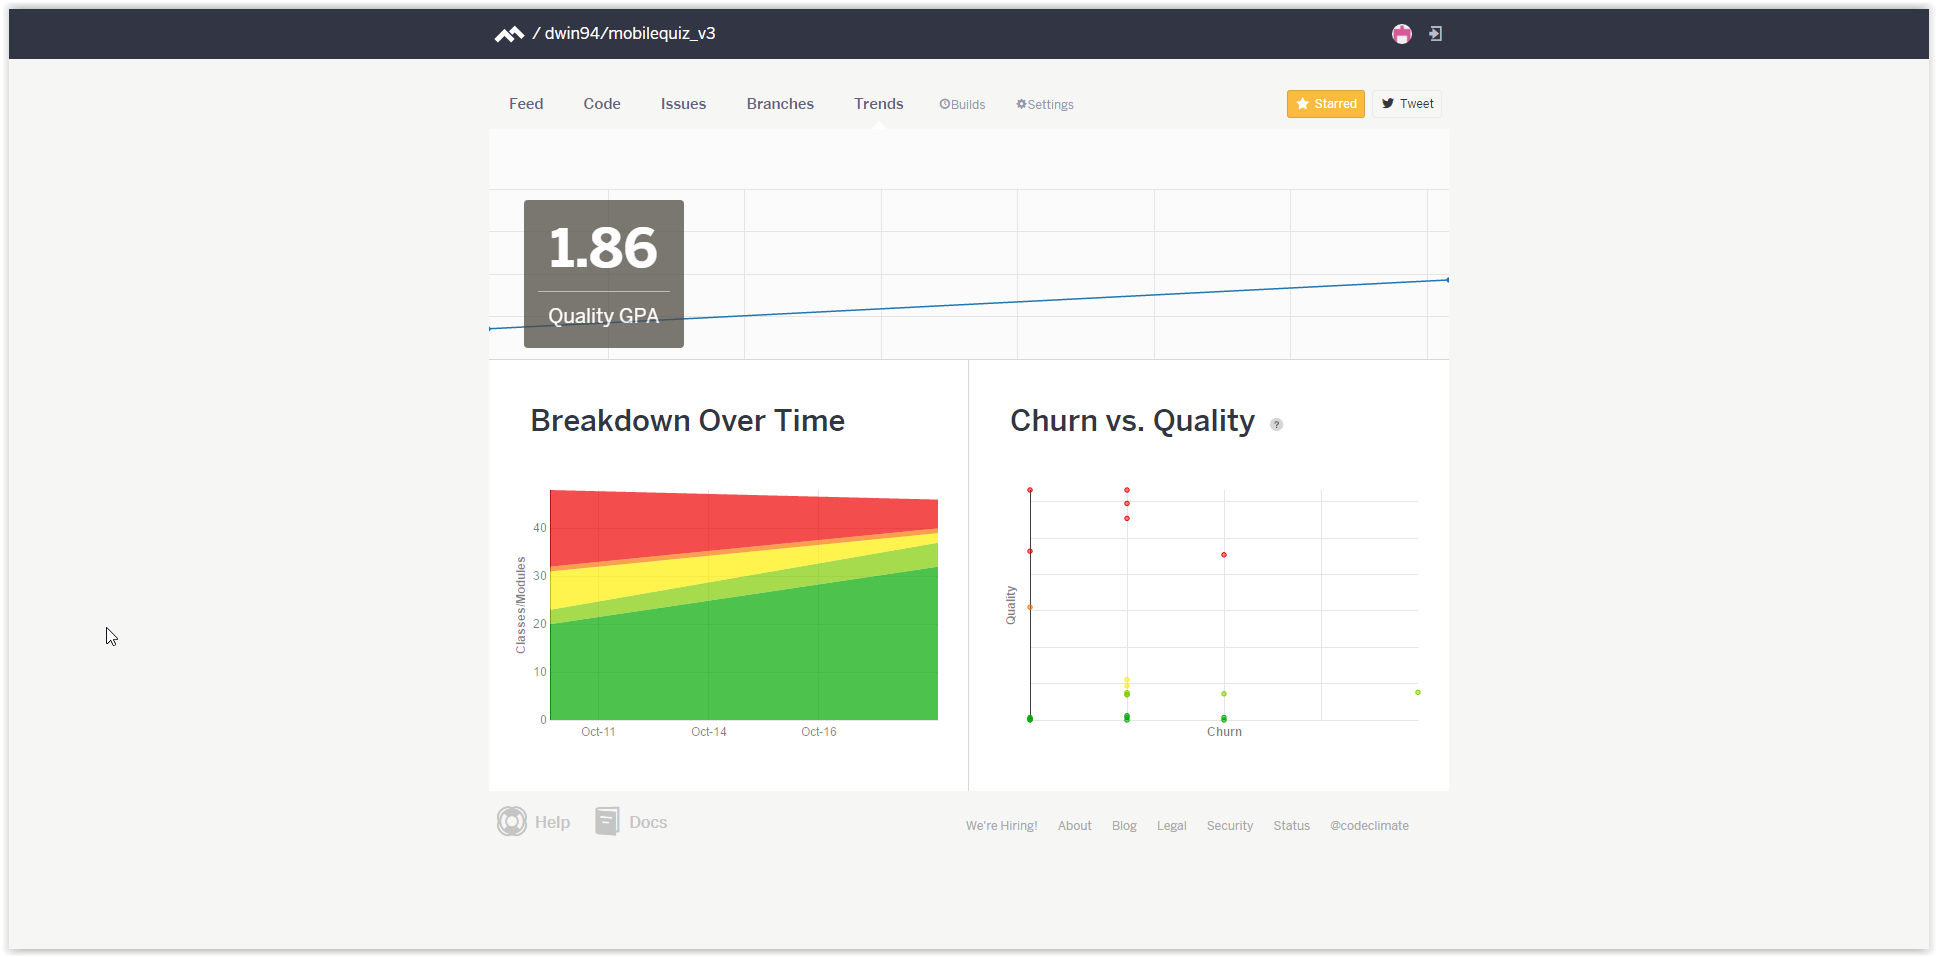
\includegraphics[width=1\textwidth
	]{Images/Stand_Beginn_181016.PNG}
	\caption{Code Climate Stand 18.10.2016 - nach der Verfeinerung der Regeln}
\end{figure}


\section{Systemtests mit Selenium}
%automatisierte Systemtests mit Selenium
Selenium IDE ist ein Firefox AddOn für Web-\acrfull{UI}-Tests. Es ermöglicht das Aufnehmen, die Bearbeitung, das Debuggen und das Abspielen von Tests. 

Mit der Hilfe dieses Tools können einfach \gls{User Interface} Tests durchgeführt werden.

\subsection{Methoden}
%Konkretes Vorgehen beschreiben
Mit dem Firefox Plugin von Selenium können die Abläufe die getestet werden sollen einfach aufgenommen werden. Das heisst der Benutzer spielt den korrekten Ablauf durch. Das einzige was von Hand gemacht werden muss, ist das assert-Statement, also die Prüfung, ob der Test korrekt durchgelaufen ist.

Alle erfassten Tests werden abgespeichert und können danach einfach abgespielt werden.

\subsection{Erkenntnisse}
%Was haben wir mit Hilfe von (siehe Titel) herausgefunden und wie werden wir es verbessern?
%Folgen sobald das Tool konkret eingesetzt wurde

\section{Code Review}
%Code Review mit GitHub Branch
%Einleitung
Mit einem Code Review wird die Codequalität sichergestellt. Dabei schaut sich jeweils derjenige, welcher den Code nicht geschrieben, den Code des anderen an. 


\subsection{Methoden}
%Konkretes Vorgehen beschreiben
Die Code Reviews wurden mit Github Branches gemacht. Das heisst der Entwickler eröffnet für seine neuen Features ein Github Branch und bevor dieser wieder in den Master merged werden kann, schaut sich das andere Teammitglied den Branch an und gibt in frei.

\subsection{Erkenntnisse}
%Was haben wir mit Hilfe von (siehe Titel) herausgefunden und wie werden wir es verbessern?
%Folgen sobald konkret eingesetzt wurde

\section{Unit-Tests}
%Unit-Tests mit PHPUnit
%Einleitung
Die Unit-Tests sind dazu da, einzelne Funktionen zu testen. Wenn eine Basis von Unit-Test bestehen, welche die Funktionalität des Codes abdecken, kann gut Refactoring betrieben werden. 

\subsection{Methoden}
%Konkretes Vorgehen beschreiben
Das Testen wurde mit PHPUnit umgesetzt. Diese Test werden bei jedem commit automatisch vom Continuous Integration Server, in unserem Fall Travis CI, ausgeführt. So wird bei jedem commit geschaut, ob noch alles funktioniert

\subsection{Erkenntnisse}
%Was haben wir mit Hilfe von (siehe Titel) herausgefunden und wie werden wir es verbessern?
%Folgen sobald konkret eingesetzt wurde




	
	
	\chapter{Schlussfolgerung}
	%Die Schlussfolgerungen bilden zusammen mit der Kurzzusammenfassung (Abstract) und der Zusammenfassung (Mgmt Summary, Broschürentext) die wichtigsten Abschnitte eines Berichts und sollen daher am sorgfältigsten ausgearbeitet sein.
	
	%·         Die Schlussfolgerungen enthalten eine Zusammenfassung und Beurteilung der Resultate (Vergleich mit anderen Lösungen, was wurde erreicht, was nicht, was bleibt noch zu tun, was würde man nun anders tun).
	%·         Bei Systementwicklungen kann eine Vergleichstabelle sinnvoll sein, welche die wichtigsten Funktionen im Vergleich zu verschiedenen Lösungen zeigt.
	%·         In den Schlussfolgerungen soll auch ein Ausblick auf das weitere Vorgehen bzw. auf die Bedeutung der erreichten Ergebnisse gegeben werden.
	
	
	
	
	
	\chapter{Literaturverzeichnis}
	%Im Literaturverzeichnis sind alle verwendeten Quellen (Bücher, Publikationen, Application Notes, Links (url), sowie Hinweise auf Gespräche mit bestimmten Personen) aufgeführt. Typischerweise werden die Quellenangaben nummeriert (z.B. [1], [2]) und in der Reihenfolge geordnet, wie sie im Bericht vorkommen. Man kann die Quellen auch mit den (abgekürzten) Namen der Autoren und dem Erscheinungsjahr bezeichnen (z.B. [Schueli90], [Shannon49]), wobei die Einträge dann alphabetisch geordnet werden. Jede Referenz ist so anzugeben, dass sie einfach auffindbar ist (evtl. inklusive Seitenzahl, Bibliothek Bestellnummer). Eine Referenz, welche die allgemeine Grundlage für ein ganzes Kapitel bildet, wird im Titel bzw. in einer Fussnote aufgeführt. Für Referenzen aus dem Internet soll ein kommentierter URL angegeben werden.
	
	%Beispiele zu Quellenangaben:
	%[1] C.E.Shannon, Communication in the Presence of Noise, Proceedings IRE, Vol. 37, January, 1949, pp. 10-21.
	%[2] Telefonat vom 22.5.92 mit Herrn XY, Firma, Adresse, Telefon-Nummer.
	%[3] 12 Tipps für einen guten Sprach- und Schreibstil  www.redenwelt.de zuletzt besucht am 15.9.2015.
	
	\bibliographystyle{IEEEtran}
	\bibliography{zotero}
	
	
	\chapter{Abkürzungsverzeichnis (Glossar)}
	%Das Abhkürzungsverzeichnis (Glossar) enthält alle im Bericht vorkommenden Abkürzungen in alphabetischer Reihenfolge. Häufig wird hier auch eine Kurzbeschreibung zu den Begriffen angegeben. In diesem Fall nennt man den Abschnitt eher "Glossar".
	
	\printglossaries
	
	
	\chapter{Abbildungsverzeichnis}
	\listoffigures
	
	
	
	\part{Anhang}
	%Der Anhang enthält Abschnitte, welche den Rahmen oder die Kontinuität der Hauptkapitel stören, da sie nicht von zentraler Bedeutung für die Endlösung sind. Auch administrative Teile der Arbeit, welche von der Schule gefordert, für das Verständnis des Endergebnisses der Arbeit weniger wichtig sind, sollen im Anhang aufgeführt sein. Die im folgenden hervorgehobenen Punkte müssen in jeder Arbeit enthalten sein, die übrigen Punkte können je nach Situation vorkommen oder nicht.
	
	
	\chapter{Persönliche Berichte zur Arbeit}
	%Persönliche Berichte zur Arbeit (wie von HSR verlangt)
	
	\chapter{Details zu Diagrammen}
	%Details zu Diagrammen (z.B. detaillierte Klassendiagramme, Sequenzdiagramme, Programmlistings, Use Cases)
	
	\chapter{Details zur Lösungsfindung}
	%Details zur Lösungsfindung (z.B. Analyseschritte, Designschritte, umfangreiche Herleitungen, Tabellen, Messergebnisse, Testauswertungen)
	
	\chapter{User Interface Abklärungen, Mockups, Paper Prototypen}
	%User Interface Abklärungen, Mockups, Paper Prototypen
	
	\chapter{Projektmanagementplan}
	%Projektmanagementplan (kommentierter Arbeitsplan, Zeiterfassung: Durch den Einbezug des Arbeitsplans in den Bericht sollen die Studenten zu einer bewussten Arbeitsplanung animiert werden, sodass sie lernen den Arbeitsaufwand abzuschätzen und die Arbeit optimal zu organisieren.
	% !TEX root = Projektdokumentation.tex

 \section{Kostenvoranschlag}
 Das Projekt läuft im Rahmen der Studienarbeit. Diese sieht einen Personenaufwand von 240 Stunden pro Person vor, was bei einer 2-Personen-Gruppe einen Aufwand von 480 Stunden macht. 
 Der Projektrahmen ist das Herbstsemester 2016, welches vom 19.09 - 23.12.2016 dauert und somit 14 Wochen umfasst. Es ist damit ein durchschnittlicher Wochenaufwand von 17 Stunden pro Person vorgesehen.
 
 
 \section{Zeitliche Planung}
 
 \subsection{Phasen / Iterationen}
 Das Projekt ist in die Phasen Inception, Elaboration, Construction und Transition aufgeteilt. Die Inception-Phase hat bereits in der Woche vor dem Semesterbeginn stattgefunden. Die restlichen Phasen sind, wie in der Grafik auf der nächsten Seite ersichtlich, über das Herbstsemesters 2017 verteilt.
 
 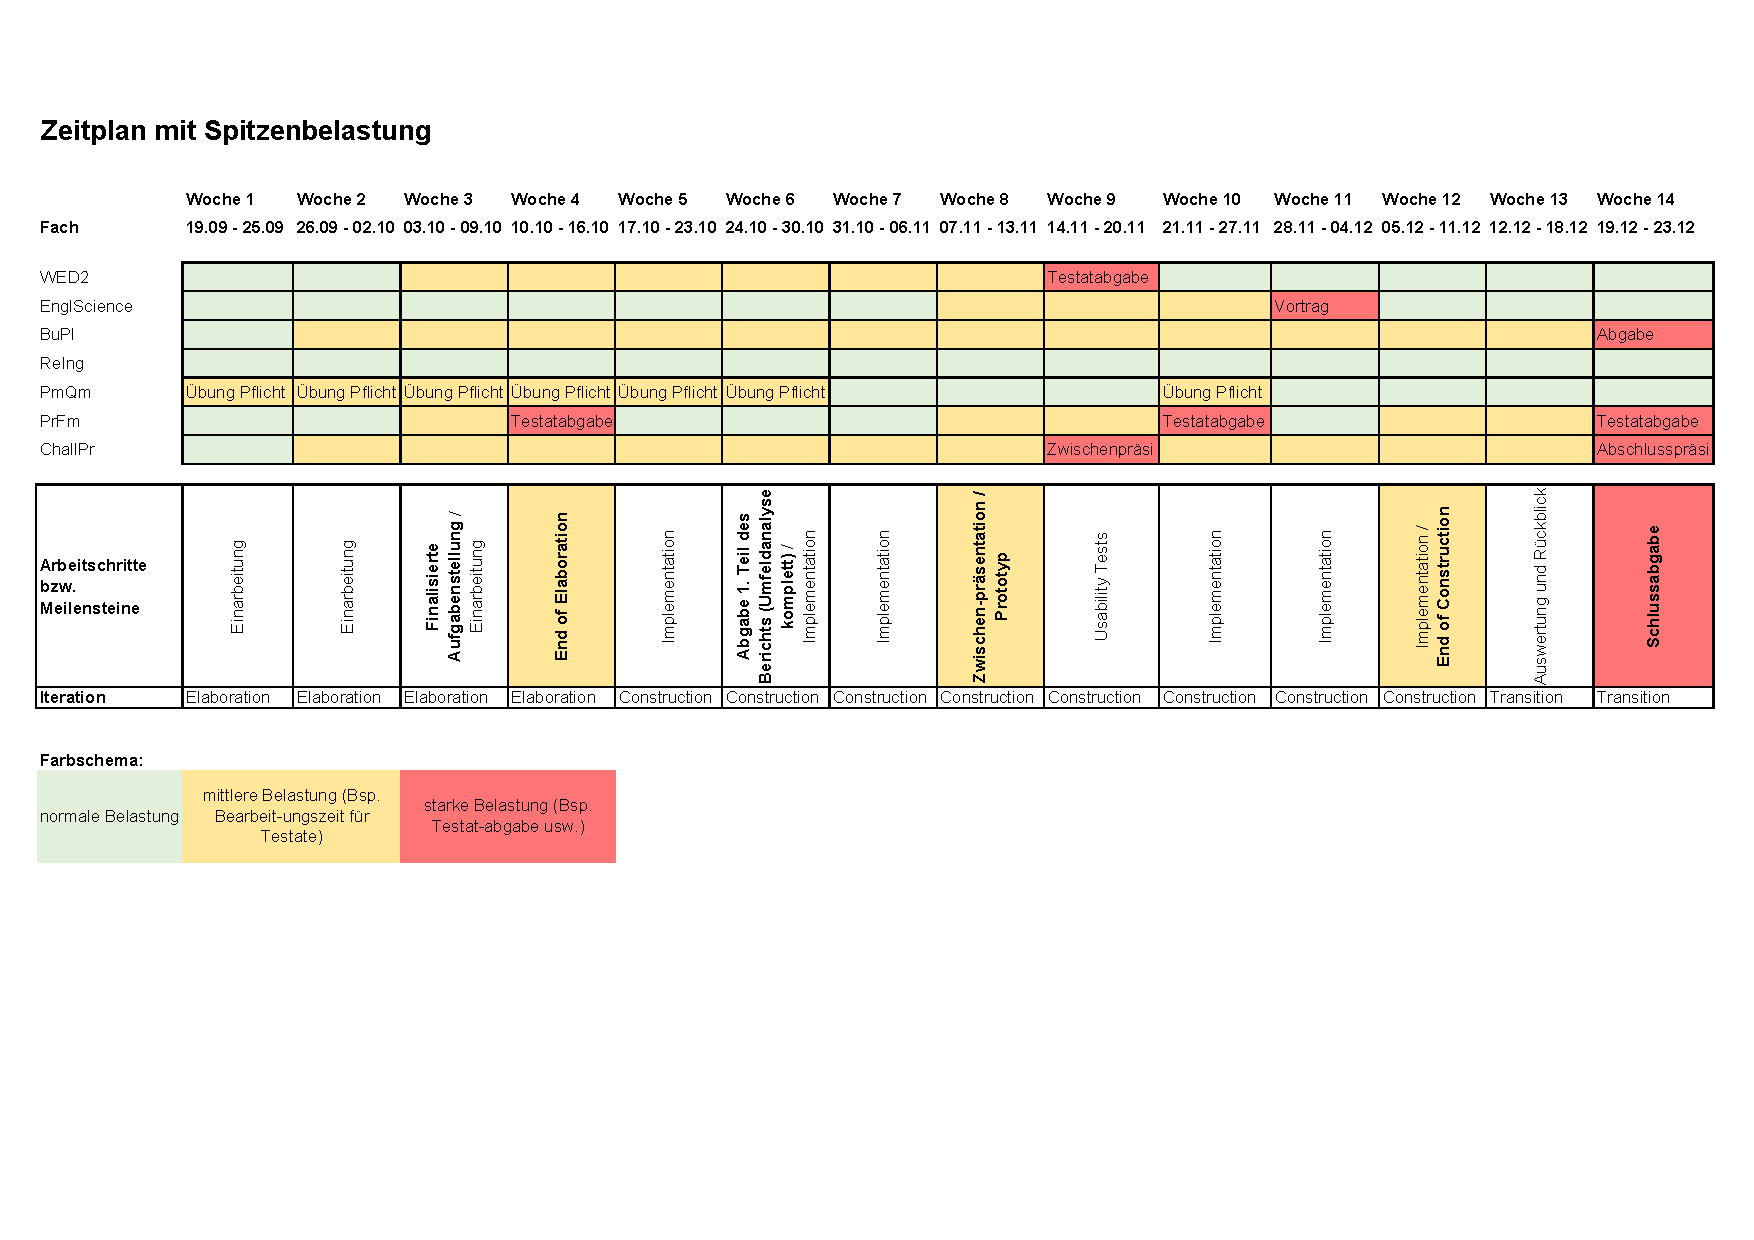
\includepdf[landscape=true]{Zeitplan_Spitzenbelastung.pdf}
 \todo{David Plan anpassen}
 
 \subsection{Meilensteine}
 
 %Die Meilensteine sollen konkret und messbar dargestellt werden.
 
 \begin{tabularx}{\linewidth}{|X|c|X|}
 	\hline
 	\textbf{Meilenstein} & \textbf{Datum} & \textbf{Beschreibung} \\
 	\hline
 	Finalisierte Aufgabenstellung & 09.10.2016 & Herr Heinzmann hat die zu erledigenden Arbeiten in einer Aufgabenstellung zusammengestellt und an die Studenten abgegeben. \\
 	\hline
 	End of Elaboration & 16.10.2016 & Die Umfeldanalyse ist abgeschlossen und es ist bekannt, welche Arbeiten im Rahmen der Studienarbeit angegangen werden. \\
 	\hline
 	Erster Teil des Berichts komplett & 30.10.2016 & Die Ergebnisse der Analyse-Phase sind vollständig niedergeschrieben, damit Herr Heinzmann diese gegenlesen kann. \\
 	\hline
 	Zwischenpräsentation & 13.11.2016 & Die bisher erarbeiteten Ergebnisse wurden Herrn Heinzmann als Vortrag präsentiert. \\
 	\hline
 	Erster Prototyp & 13.11.2016 & Die Code-Änderungen für eine verbesserte Usability wurden vollständig implementiert, damit in der Folgewoche die zweiten Usability-Tests durchgeführt werden können. \\
 	\hline
 	End of Construction & 11.12.2016 & Alle Änderungen am Code wurden implementiert, sodass dieser wieder auf den cnlab-Server übertragen werden kann. \\
 	\hline
 	Schlussabgabe & 23.12.2016 & Alle Dokumente wurden abgabekonform erstellt, die Dokumentation gebunden, der Code auf CD gebrannt und alles an Herrn Heinzmann abgegeben. \\
 	\hline
 \end{tabularx}
 
 
 
 \section{Zeiterfassung}
 Für alle Arbeiten werden in Redmine Arbeitspakete erfasst. Sofort nachdem ein Paket bearbeitet wurde, wird die Zeit darauf verbucht. Da alle Pakete einer Kategorie zugeordnet sind, kann am Ende des Projekts genau festgestellt werden, wie viel Zeit beispielsweise für alle Dokumentationen aufgewendet wurde.
 
 Die bereits erfassten Pakete sowie deren Fortschritt sind auf den folgenden Seiten abgebildet:
 
 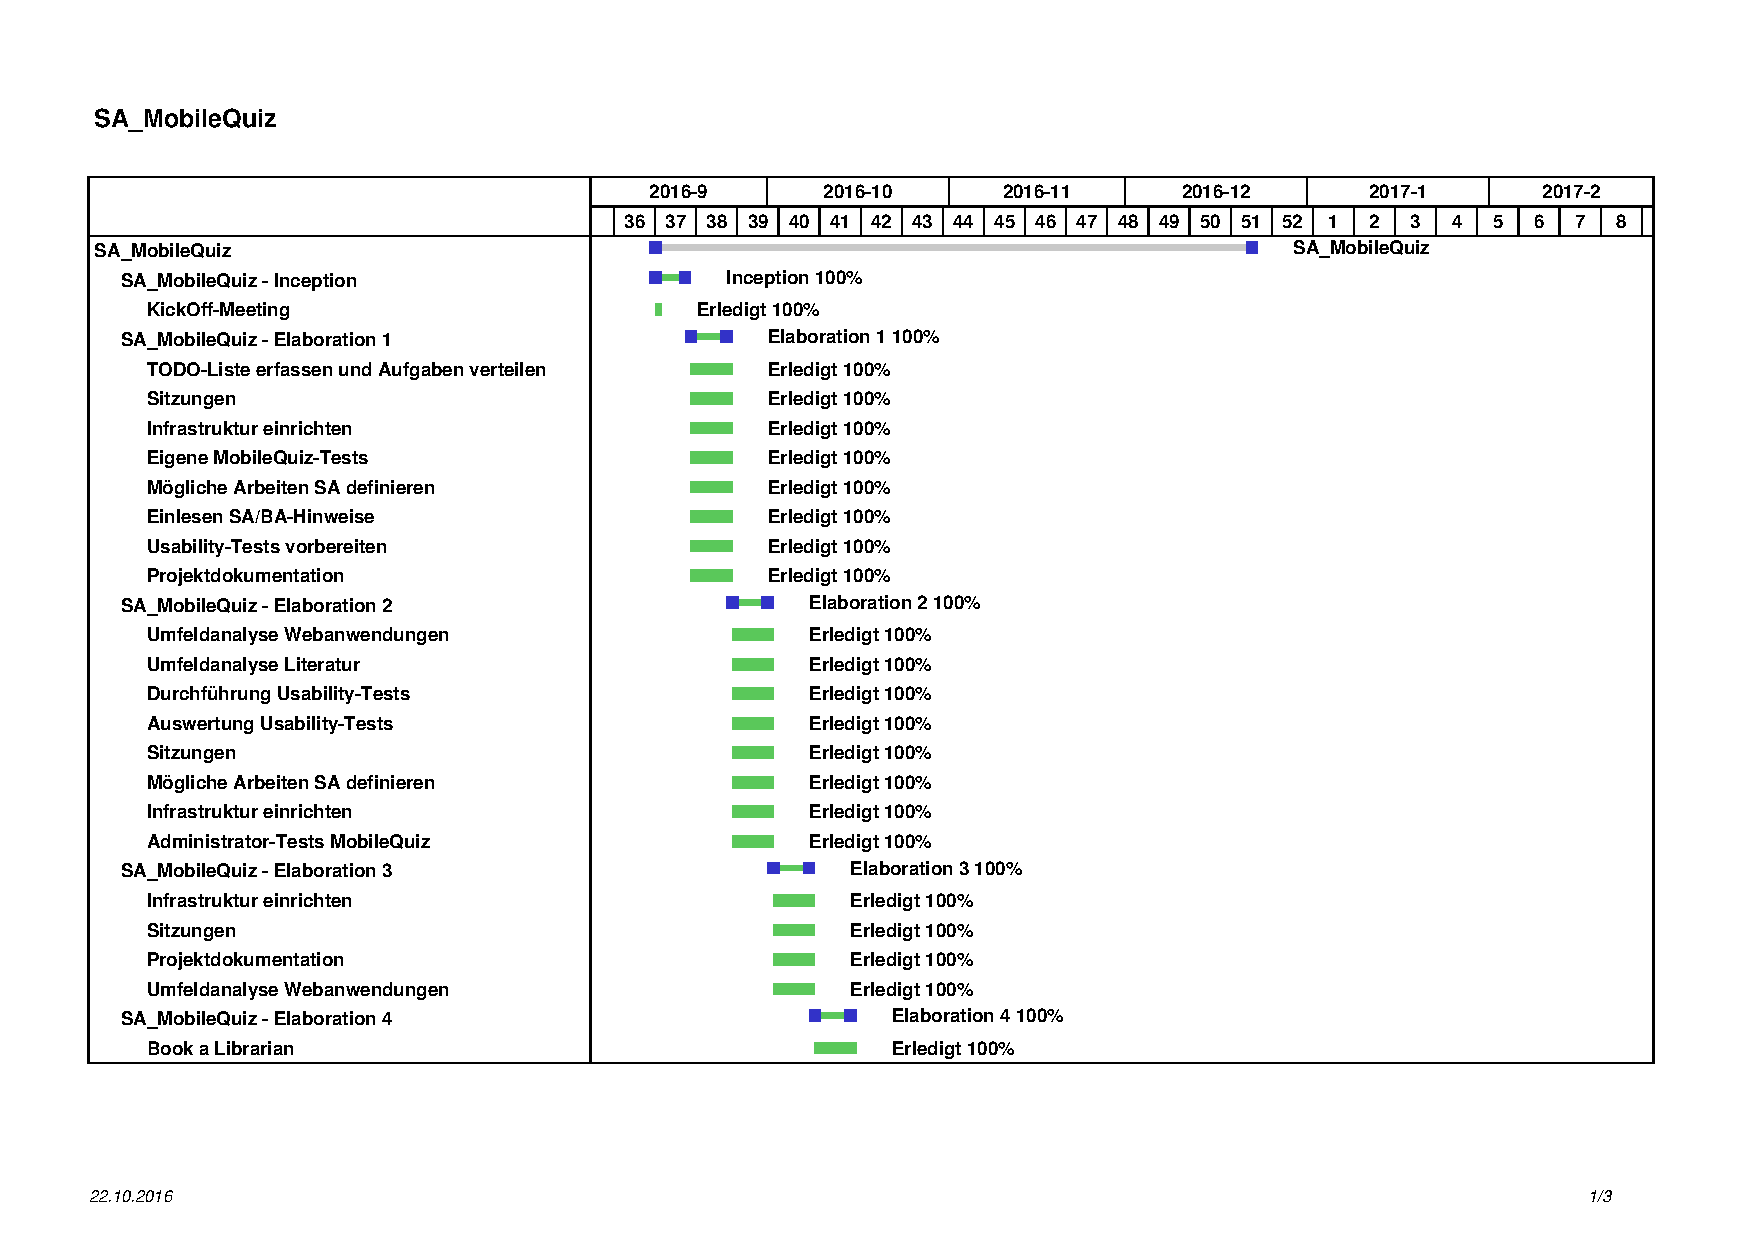
\includepdf[landscape=true,pages={1-3}]{sa_mobilequiz-gantt_22-10-2016.pdf}
	
	\todo{David}
	
	\chapter{Risikomanagement}
	%Bezug nehmen auf das Excel.
	Eine Übersicht aller technischen Risiken befindet sich auf der folgenden Seite. Darin ist der aktuelle Zustand aller uns bekannten Risiken ersichtlich.
	
	\section{Umgang mit Risiken}
	Die Teammitglieder sind bereit, bei unerwarteten oder nicht vorhergesehenen Zwischenfällen das Arbeitspensum für die Studienarbeit zu erhöhen, um den fristgerechten Abschluss der Arbeit zu gewährleisten, solange es sich dabei nicht um einen Dauerzustand handelt. Zusätzlich wird bei der Schätzung der Aufwände immer darauf geachtet, für unerwartetes eine Reserve einzuplanen.
	Nach jeder Iteration werden die bestehenden Risiken neu evaluiert und falls nötig angepasst oder neue Risiken aufgenommen.
	
	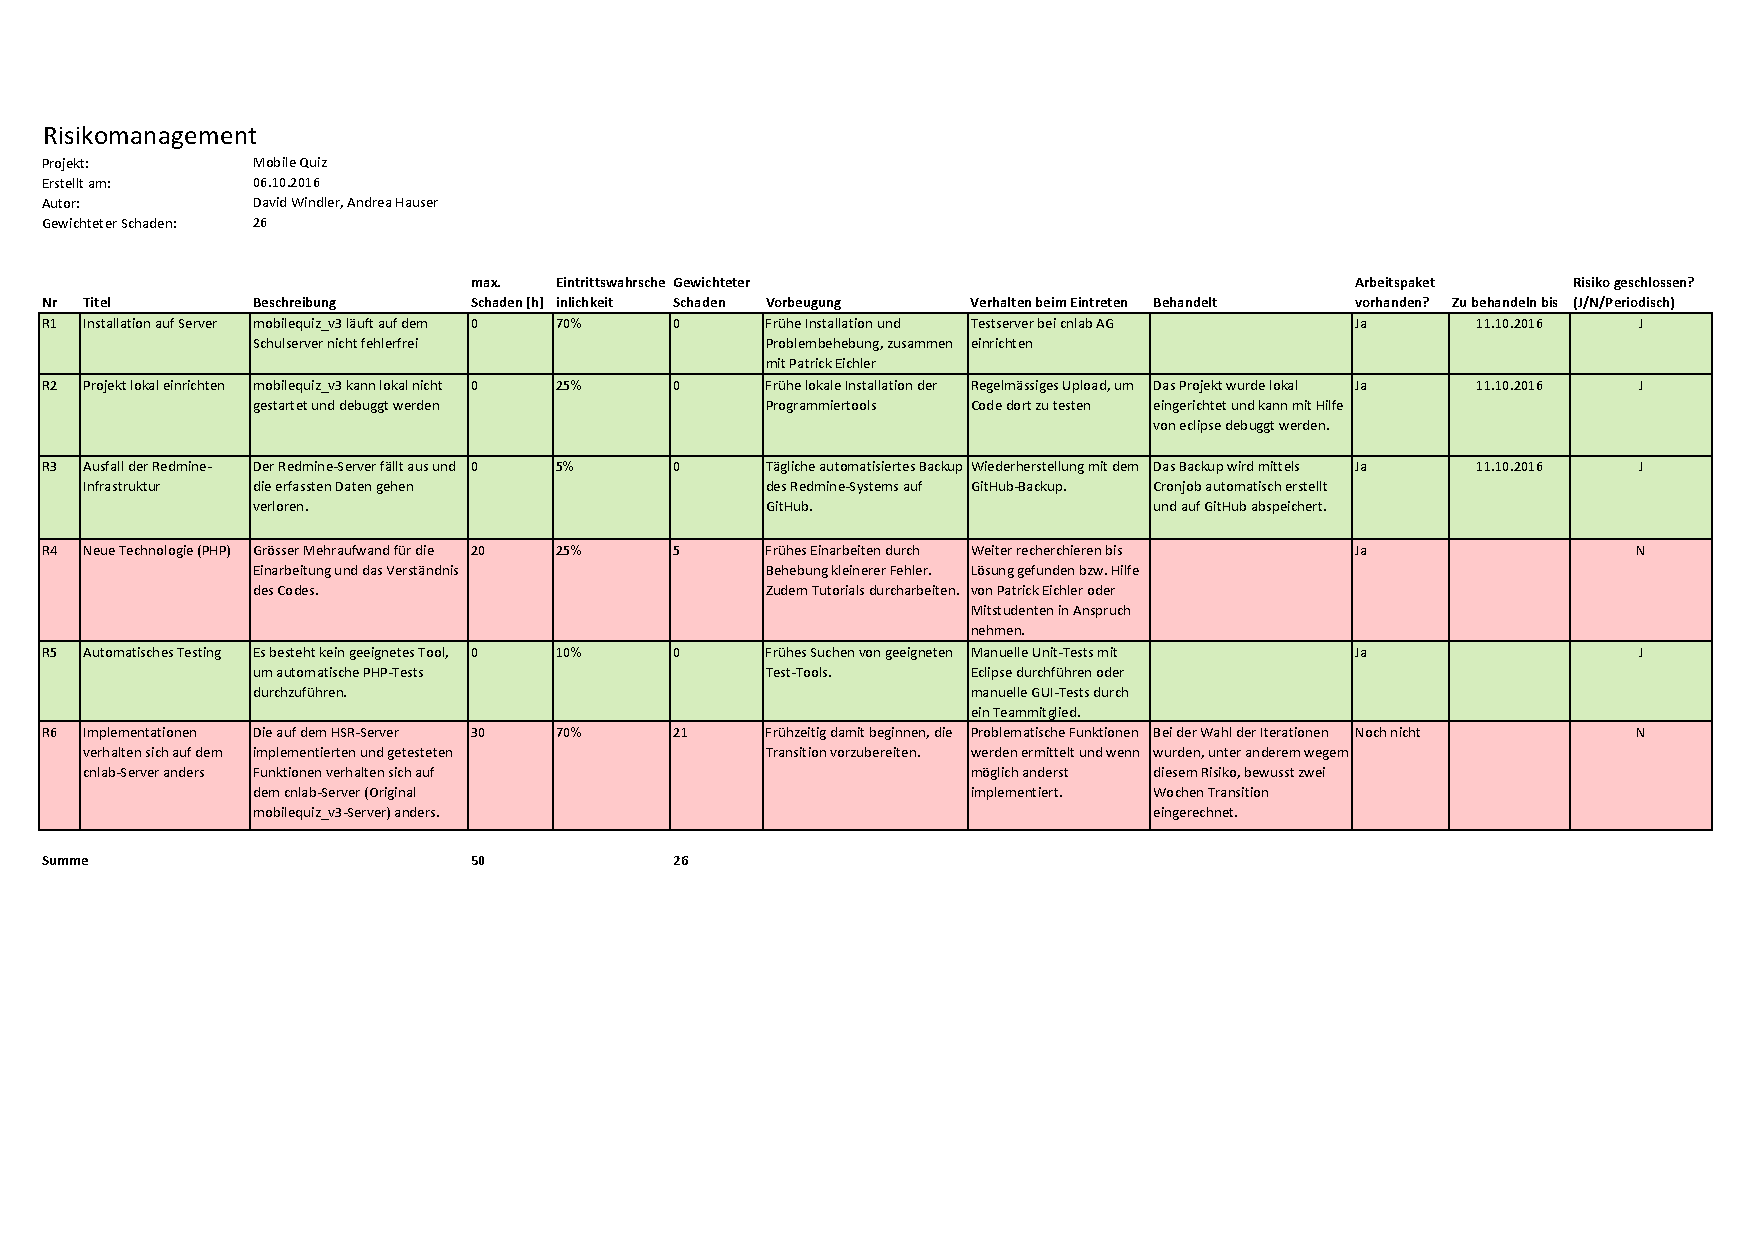
\includepdf[landscape=true]{TechnischeRisiken.pdf} 

	\chapter{Verwendete Werkzeuge}
	% !TEX root = Projektdokumentation.tex

\section{Dokumentenverwaltung}

\begin{description}
	\item [OneDrive] ist ein Dienst von Microsoft, um Dateien auf einem zentralen Speicherort abzulegen. Auf diesen kann über das Internet zugegriffen werden. \cite{wikipedia_filehosting} \cite{wikipedia_oneDrive}
	\begin{itemize}
		\item Einsatzzweck: Dokumentenablage
		\item Version: 17.3
		\item Bezugsquelle: https://onedrive.live.com/about/de-de/download/
		\item Beachten: Benötigt kostenlose Registrierung auf https://onedrive.live.com/
	\end{itemize}
	
	
	\item [GitHub] ist ein Online Versionsverwaltungssystem für Software.
	\begin{itemize}
		\item Einsatzzweck: Versionskontrolle für Code und Latex-Projektdokumentation
		\item Version: unbekannt
		\item Webseite: https://github.com/
		\item Beachten: Benötigt kostenlose Registrierung auf https://github.com/join. Gratis Private-Repositories gibt es als Studenten mit der Registrierung auf https://education.github.com/pack
	\end{itemize}
	
	
	\item [GitHub Desktop] ist ein Programm für Windows und macOS, um GitHub-Repositories zu lokal synchronisieren und verwalten.
	\begin{itemize}
		\item Einsatzzweck: Synchronisation von Code und Latex-Projektdokumentation
		\item Version: 3.3.1.0
		\item Bezugsquelle: https://desktop.github.com/
	\end{itemize}
\end{description}



\newpage
\section{Server-Zugriff}

\begin{description}
	\item [FileZilla Client] ist ein Programm für Windows, macOS und Linux, um mittels FTP (File Transfer Protocol) Daten auf einen Server hoch- und herunterzuladen. \cite{wikipedia_filezilla}
	\begin{itemize}
		\item Einsatzzweck: Dateien auf HSR-Server hochladen
		\item Version: 3.22.1
		\item Bezugsquelle: http://filezilla.de/
	\end{itemize}
	
	
	\item [PuTTY] ist ein Programm für Windows und Linux, um Verbindungen mittels SSH (Secure Shell), Telnet oder über eine serielle Schnittstelle herzustellen. \cite{wikipedia_putty}
	\begin{itemize}
		\item Einsatzzweck: SSH-Verbindung zum HSR-Server, um Installationen oder Konfigurationen vorzunehmen.
		\item Version: 0.67
		\item Bezugsquelle: http://www.putty.org/
	\end{itemize}
\end{description}



\section{Projektverwaltung}

\begin{description}
	\item [Redmine] ist eine web-basierte Projektmanagement-Software.
	\begin{itemize}
		\item Einsatzzweck: Projektplanung, Ticketverwaltung und Zeiterfassung
		\item Version: 3.3.0.stable
		\item Bezugsquelle: Von Schule vorinstalliert.
	\end{itemize}
\end{description}


\newpage
\section{Dokumentation}

\begin{description}
	\item [Microsoft Office] ist ein Paket von Büro-Software für Windows, macOS, iOS, Android und Windows Phone. \cite{wikipedia_microsoft-office}
	\begin{itemize}
		\item Einsatzzweck: Dokumenten- und Tabellenerstellung, ausser Projektdokumentation
		\item Version: 1609
		\item Bezugsquelle: https://products.office.com/
		\item Beachten: Das Office-Paket kann als HSR-Student kostenlos heruntergeladen werden.
	\end{itemize}
	
	
	\item [TeXstudio] ist ein LaTex-Editor für Windows, macOS und Linux.
	\begin{itemize}
		\item Einsatzzweck: Erstellung von LaTex-Dokumenten, vor allem für Projektdokumentation
		\item Version: 2.11.0
		\item Bezugsquelle: http://www.texstudio.org/
		\item Beachten: Für die Erstellung von LaTex-Dokumenten benötigt es eine TeX-Distribution (siehe MiKTeX). Weiter ist ein Perl-Interpreter Voraussetzung, um ein Glossar zu erstellen.
	\end{itemize}
	
	
	\item [MiKTeX] ist eine TeX-Distribution für Windows. \cite{wikipedia_miktex}
	\begin{itemize}
		\item Einsatzzweck: Interpretation und Kompilation von LaTex-Dokumenten
		\item Version: 2.9
		\item Bezugsquelle: https://miktex.org/download
	\end{itemize}
	
	
	\item [ActivePerl] ist ein Perl-Interpreter für Windows.
	\begin{itemize}
		\item Einsatzzweck: Erstellung von LaTex-Glossaren
		\item Version: 5.24.0
		\item Bezugsquelle: http://www.activestate.com/activeperl
	\end{itemize}
	
	
	\item [Zotero] ist eine Quellenverwaltungs-Software für Windows, macOS und Linux.
	\begin{itemize}
		\item Einsatzzweck: Quellenverwaltung
		\item Version: 4.0.29.10
		\item Bezugsquelle: https://www.zotero.org/download/
		\item Beachten: Für das Speichern von neuen Quellen eignet sich das Browser-AddOn. Weiter können die Exporteinstellungen des Zotero-Standalone auf BibTeX eingestellt werden, was es ermöglicht, neue Quellen per Drag\&Drop einer .bib-Datei hinzuzufügen. So können neue Quellen schnell und einfach in LaTeX eingebunden werden.
	\end{itemize}
\end{description}



\section{Software-Entwicklung}

\begin{description}
	\item [PHP Eclipse] ist eine PHP-Entwicklungsumgebung für Windows, macOS und Linux.
	\begin{itemize}
		\item Einsatzzweck: PHP-Entwicklung
		\item Version: Neon.1 Release (4.6.1)
		\item Bezugsquelle: https://eclipse.org/pdt/
	\end{itemize}	
	
	
	\item [XAMPP Control Panel] ist eine PHP-Entwicklungsumgebung für Windows, macOS und Linux. Sie enthält Apache, MariaDB, PHP und Perl.
	\begin{itemize}
		\item Einsatzzweck: Lokale PHP-Entwicklung und Debugging. Über phpMyAdmin konnte die Datenbank leicht lokal installiert werden. Weiter ist der Apache-Server schnell eingerichtet. Da der Eclipse-Workspace im htdocs von Apache liegt, können Änderungen sofort nachvollzogen werden. Zudem ermöglicht die Kombination mit easy Xdebug (s. unten) ein einfaches Debugging mit Firefox und Eclipse.
		\item Version: 3.2.2
		\item Bezugsquelle: https://www.apachefriends.org/de/index.html
	\end{itemize}
	
	
	\item [easy Xdebug (with moveable icon)] ist ein Firefox AddOn, um einfaches Debugging mittels Eclipse zu ermöglichen.
	\begin{itemize}
		\item Einsatzzweck: Debugging mit Eclipse
		\item Version: 0.9.4
		\item Bezugsquelle: https://addons.mozilla.org/de/firefox/addon/easy-xdebug-with-moveable-
		\item Beachten: Es ist folgendermassen vorzugehen, um PHP mit Eclipse zu debuggen:
		\begin{enumerate}
			\item XAMPP Control Panel: Start von MySQL und Apache
			\item Start von Eclipse und Öffnen des Projekts
			\item Start von Firefox
			\item Firefox: Aktivierung des Toggle xdebug (roter Punkt sichtbar)
			\item Firefox: Navigation zu localhost/\textless Projektname in htdocs\textgreater
			\item Nun sollte Eclipse aufleuchten und fragen, ob in den Debug-Mode umgestellt werden soll.
		\end{enumerate}
	\end{itemize}
	
	
	\item [Selenium IDE] ist ein Firefox AddOn für Web-UI-Tests. Es ermöglicht das Aufnehmen, die Bearbeiten, das Debuggen und das Abspielen von Tests.
	\begin{itemize}
		\item Einsatzzweck: Erstellen und Abspielen von Web-UI-Tests
		\item Version: 2.9.1.1
		\item Bezugsquelle: https://addons.mozilla.org/de/firefox/addon/selenium-ide/
	\end{itemize}
\end{description}



\section{Continuous Integration}

\begin{description}
	\item [Travis] ist ein Online Continuous-Integration Service für GitHub-Projekte.
	\begin{itemize}
		\item Einsatzzweck: Builden und Unit-Testen von PHP-Code
		\item Version: unbekannt
		\item Webseite: https://travis-ci.org/ und https://travis-ci.com/
		\item Beachten: Als Student mit dem GitHub Student Developer Pack kann man unter https://travis-ci.com/ Private-Repositories kostenlos builden.
	\end{itemize}
	
	
	\item [Code Climate] ist ein Online Service, um die Code-Qualität und Test-Coverage zu messen.
	\begin{itemize}
		\item Einsatzzweck: Qualitätsmessung des PHP-Codes
		\item Version: 1.0
		\item Webseite: https://codeclimate.com/
		\item Beachten: Code Climate kann mit Travis verknüpft werden. Hat Travis alle Tests durchgeführt, so leitet er dann die Ergebnisse direkt weiter. Siehe dazu die Datei '.travis.yml'. Die Konfiguration für die Qualitäts-Tests von Code Climate sind in '.codeclimate.yml' festgelegt.
	\end{itemize}
\end{description}



\section{Usability}

\begin{description}
	\item [myBalsamiq] ist ein Online Service für die Erstellung von Mockups.
	\begin{itemize}
		\item Einsatzzweck: Erstellung von Mockups
		\item Version: Build \#release/4832 - 4832
		\item Webseite: https://www.mybalsamiq.com/
		\item Beachten: Als HSR-Student kann man dem Informatik-Studiengangleiter eine Anfrage schreiben, um kostenlos ein Projekt auf myBalsamiq erstellen zu können.
	\end{itemize}
\end{description}

	
	
	\chapter{Spezielle nicht öffentlich verfügbare Berichte oder Datenblätter}
	%Spezielle nicht öffentlich verfügbare Berichte oder Datenblätter.
	
	\chapter{Passworte/Logins}
	%Passworte/Logins  (eventuell in speziellem Couvert abgegeben)
	
	\chapter{Kontaktadressen}
	%Kontaktadressen von allen beteiligten Personen (Adressen der Studenten, über welche sie auch nach der Zeit an der HSR erreicht werden können, Industriepartner, Betreuer, weitere Personen)
	\begin{multicols}{2}
	\noindent \textbf{Studenten:}
	\\
	Andrea Hauser\\
	Waldheim 1\\
	8825 Hütten\\
	E-Mail: andrea.hauser@hotmail.ch\\
	\\
	David Windler\\
	Heid 420\\
	9502 Braunau\\
	\columnbreak
	E-Mail: david.windler@windowslive.com\\
	\textbf{Betreuer:}\\
	Peter Heinzmann\\
	E-Mail: peter.heinzmann@hsr.ch\\
	\\
	Patrick Eichler\\
	E-Mail: patrick.eichler@hsr.ch\\
	
	\end{multicols}
	
	
	\chapter{Inhaltsverzeichnis zur mit der Arbeit abgegeben CDROM}
	%Inhaltsverzeichnis zur mit der Arbeit abgegeben CDROM
	%Diese kann beispielsweise folgende Teile enthalten:
	%·         Gesamten Code
	%·         Alle Dokumente der Arbeit (in Originalformat und als PDF)
	%·         Alle Präsentationen zur Arbeit (in Originalformat bzw. Powerpoint und/oder PDF)
	%·         Reviews, Zwischenberichte
	%·         Sitzungsprotokolle
	%·         Protokolle zu Telefonaten, spezielle Mails
	
	
	
	
	
	
	
	
	
	
\end{document}